% !TeX program = xelatex 
\documentclass{hitreport}
\usepackage{url}
\usepackage{algorithm,float}  
\usepackage{algpseudocode}  
\usepackage{amsmath}
\usepackage{cite}
\usepackage{threeparttable}
\usepackage{subfig}
\usepackage{listings} %插入代码
\usepackage{xcolor} %代码高亮
\usepackage{tikz}
\usepackage{hyperref}
\usepackage{wasysym}
\usepackage{pgfplots}
\usetikzlibrary{positioning}




\lstset{numbers=left, %设置行号位置
	numberstyle=\tiny, %设置行号大小
	keywordstyle=\color{blue}, %设置关键字颜色
	commentstyle=\color[cmyk]{1,0,1,0}, %设置注释颜色
	frame=single, %设置边框格式
	escapeinside=``, %逃逸字符(1左面的键),用于显示中文
	breaklines, %自动折行
	extendedchars=false, %解决代码跨页时,章节标题,页眉等汉字不显示的问题
	xleftmargin=2em,xrightmargin=2em, aboveskip=1em, %设置边距
	tabsize=4, %设置tab空格数
	showspaces=false %不显示空格
}

\renewcommand{\algorithmicrequire}{\textbf{Input:}}  % Use Input in the format of Algorithm  
\renewcommand{\algorithmicensure}{\textbf{Output:}} % Use Output in the format of Algorithm  

\makeatletter
\newenvironment{breakablealgorithm}
  {% \begin{breakablealgorithm}
   \begin{center}
     \refstepcounter{algorithm}% New algorithm
     \hrule height.8pt depth0pt \kern2pt% \@fs@pre for \@fs@ruled
     \renewcommand{\caption}[2][\relax]{% Make a new \caption
       {\raggedright\textbf{\ALG@name~\thealgorithm} ##2\par}%
       \ifx\relax##1\relax % #1 is \relax
         \addcontentsline{loa}{algorithm}{\protect\numberline{\thealgorithm}##2}%
       \else % #1 is not \relax
         \addcontentsline{loa}{algorithm}{\protect\numberline{\thealgorithm}##1}%
       \fi
       \kern2pt\hrule\kern2pt
     }
  }{% \end{breakablealgorithm}
     \kern2pt\hrule\relax% \@fs@post for \@fs@ruled
   \end{center}
  }
\makeatother

% =============================================
% Part 0 Edit the info
% =============================================

\major{计算机科学与技术}
\name{孙骁}
\title{认知神经科学原理\\实验报告}
\stuid{1180300811} % 学号
\college{计算学部}
\date{\today}
\lab{格物213} %实验地点
\course{认知神经科学原理}
\instructor{马琳}
% \grades{}
\expname{信息相关电位认知实验\\听觉Oddball实验} %实验名称
% \exptype{} % 实验类型
% \partner{} % 同组学生名字
\term{2020秋季学期}

\begin{document}

\maketitle

\tableofcontents
\newpage
% =============================================
% Part 1 Header
% =============================================



% =============================================
% Part 2 Main document
% =============================================

\section{ERPs定义及性质}

首先介绍诱发电位(Evoked Potentials, EPs),也称为诱发反应,是指给予神经系统特定的刺激,或使大脑对刺激的信息进行加工,在该系统和脑的相应部位产生的可以检出的、与刺激有相对固定时间间隔和特定位相的生物电反应\cite{LEGATT2014228}。

ERP(Event-Related Potential)即事件相关电位\cite{Sur2009},是一种特殊的脑诱发电位,是大脑的特定脑区在受到不同刺激时记录的电位变化。ERP研究方法是将刺激事件,包括:视觉、听觉、体感等物理刺激和心理因素,在大脑内引起的相关反应,客观的表达出来,为观察认知活动在不同时间进程中的脑功能活动状态,研究人类心理和行为的神经机制,以及认知的发展、成熟、衰退过程提供可靠的实验技术方法\cite{Luck2014}。

ERP的性质如下:

\begin{enumerate}
\item ERPs不像普通诱发电位记录神经系统对刺激本身产生的反应,而是大脑对刺激带来的信息引起的反应\cite{Sur2009}。是在注意的基础上,与识别、比较、判断、记忆、决断等心理活动有关,反映了认知过程中大脑的神经电生理改变。
\item ERPs成分除受刺激物理特性影响的“外源性(生理性)成分”,还包括不受刺激物理特性的影响“内源性(心理性)成分”,与被试的精神状态和注意力有关\cite{Luck2014}。
\item ERPs属于长潜伏期诱发电位,测试时一般要求被试者清醒,并在一定程度上参与其中。
\end{enumerate}



\section{脑认知功能与ERPs关联关系}

\paragraph{脑认知功能}~{}

大脑的认知功能是一种心理过程,可以使我们接收,选择,存储,转换,发展和恢复从外部刺激中收到的信息\cite{Zhang1907}。这个过程使我们能够更有效地理解世界并与之建立联系。认知功能是一种基于大脑的感知技能,我们需要执行从最简单到最复杂的任何任务。它们与我们学习,记忆,解决问题和注意力的机制有关。

\paragraph{脑认知功能与ERPs的关系}~{}

借助ERPs的分析方法是研究大脑信息处理阶段认知功能的最常用的动态方法之一\cite{Luck2014}。通过使用相应工具测量相关脑区上的ERP的数据提供了有关早期感觉感知过程和更高级处理的信息,包括注意状态,皮质抑制,决策反应,错误监测,记忆更新和其他认知活动\cite{soc2017}。基于ERP的研究方法是研究典型受试者的规范性认知过程的一种有价值的技术,同时,ERP可以用作评估具有神经发育疾病的儿童(例如ASD和ADHD)\cite{soc2019}或患有各种精神病的成年个体差异的敏感工具(例如PTSD,ASD,SCZ,物质使用障碍[SUD]等)\cite{soc2018}\cite{Baruth2010}。

尽管功能性神经影像学(例如功能性磁共振成像[fMRI]或正电子发射断层扫描[PET])取得了重大进展,但因为许多精神病性疾病与可检测到的脑电图反应模式改变有关,ERP仍然是精神病学中的一种重要的大脑研究方法。ERP技术在精神病理学中可以用作功能诊断目的的有效和敏感的生物标记(例如阿尔兹海默症)\cite{Horvath2018}。另一方面,对神经发育障碍者的ERP与普通人的ERP之间差异的比较可以有助于更好地理解神经发育障碍和其他精神病学中扰乱的认知功能\cite{LAUZHU2019100635}。

\section{认知神经科学实验范式及意义}

\subsection{听觉Oddball实验及结果分析}

\subsubsection{听觉Oddball实验介绍}

\paragraph{实验目的及意义}~{}
 
探究人在加工小概率刺激时,大脑的异常反应。经典Oddball范式为在一项实验中,随机呈现作用于同一感觉通道的两种刺激,刺激出现的概率有很大差别。概率大者我们称之为标准刺激(standard stimuli),相当于是整个实验中的背景;概率小和偶然出现的刺激则为偏差刺激(deviant stimuli)。

\paragraph{实验流程}~{}
 
实验共包含两种声音刺激,两种声音刺激除音高外完全相同,两种声音出现的频率不同(高音:低音=1:4)。两种声音随机出现,被试需对两种声音刺激做出不同的按键反应。

\paragraph{问题}~{}

\begin{enumerate}
\item 计算标准刺激和偏差刺激对应的准确率以及反应时长,并进行比较和分析;
\item 分析标准刺激和偏差刺激对应的ERP差异,并测量幅值、潜伏期差异对应的脑区、电极以及时间;
\item 请检索与实验相关5篇文献综述与之相关结果。
\end{enumerate}

\paragraph{事件码}~{}
\newline
11: 2000Hz声音刺激\\
22: 500Hz声音刺激\\
1: 对2000Hz声音进行按键响应\\
2: 对500Hz声音进行按键响应

\subsubsection{听觉Oddball实验结果分析}

\paragraph{问题一}~{}\label{sec:oddballques1}

对实验数据进行预处理,得到采样频率为1000Hz的预处理实验数据,将EEG结构体的event属性导出到excel中,得到如图(\ref{fig:oddexcel})的结果。

\begin{figure}[htb]
\centering
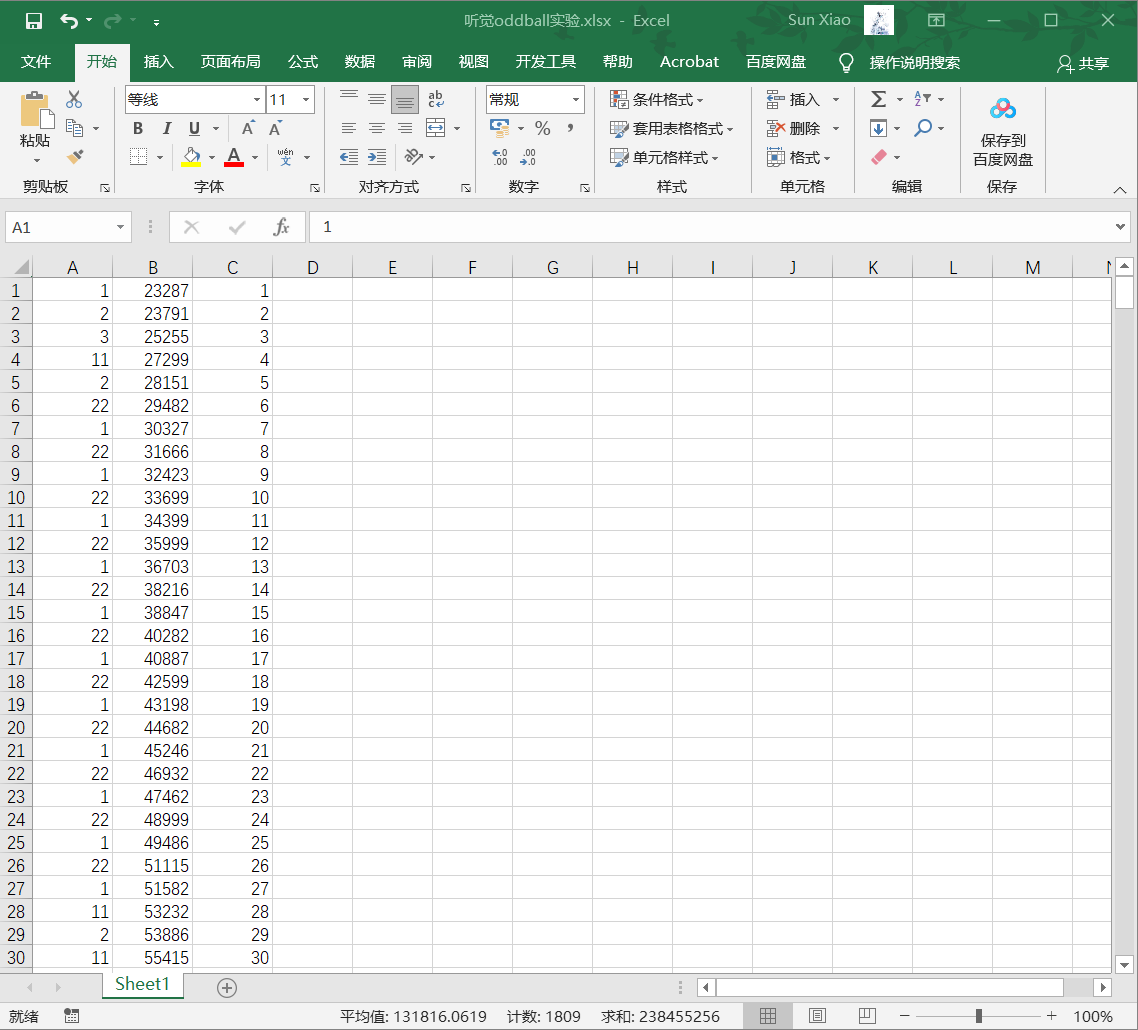
\includegraphics[scale=0.3]{oddexcel.png}
\caption{将Oddball实验的事件信息导入Excel结果}\label{fig:oddexcel}
\end{figure}

由于在实验中我对于高频和低频按键记反,所以事件码1和2正好相反。将Excel文件转化为csv文件,编写代码计算事件码11和事件码2之间以及事件码22和事件码1之间的平均反应时长,以及计算标准刺激以及偏差刺激对应的准确率。

实验的代码间附录\ref{app:oddball}

最终得到的结果如log文件所示。
\begin{lstlisting}[language=bash]
the number of high frequency(11) is 51
the number of low frequency(22) is 249
the response accuracy of high frequency(11) is 1.0
the response accuracy of low frequency(22) is 1.0
the average of reaction time of high frequency(11) is 519.843137254902
the average of reaction time of low frequency(22) is 555.6586345381526
\end{lstlisting}


高音刺激与低音刺激对应的准确率均为100\%,高音刺激的平均反应时间为519.84 ms,低音刺激的平均反应时间为555.66 ms。

\paragraph{问题二}~{}

标准刺激叠加后的ERP频谱图如图(\ref{fig:standardERP})所示,偏差刺激叠加后的ERP频谱图如图(\ref{fig:pianchaERP})所示。采样频率设置为30\%,画出的脑地形图频率为6Hz、10Hz、22Hz和40Hz,画出的频带范围是1$\sim$45Hz。

\begin{figure}[htb]
	\centering
	\subfloat[标准刺激叠加后的ERP频谱图]{\label{fig:standardERP}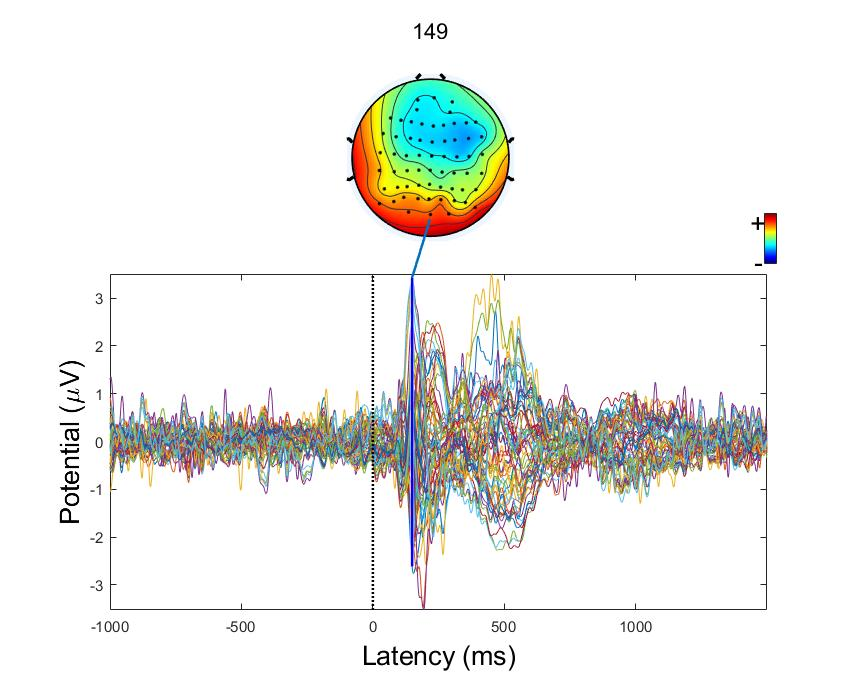
\includegraphics[scale=0.2]{listen_erp_22.jpg}}\hspace{5pt}
	\subfloat[偏差刺激叠加后的ERP频谱图]{\label{fig:pianchaERP}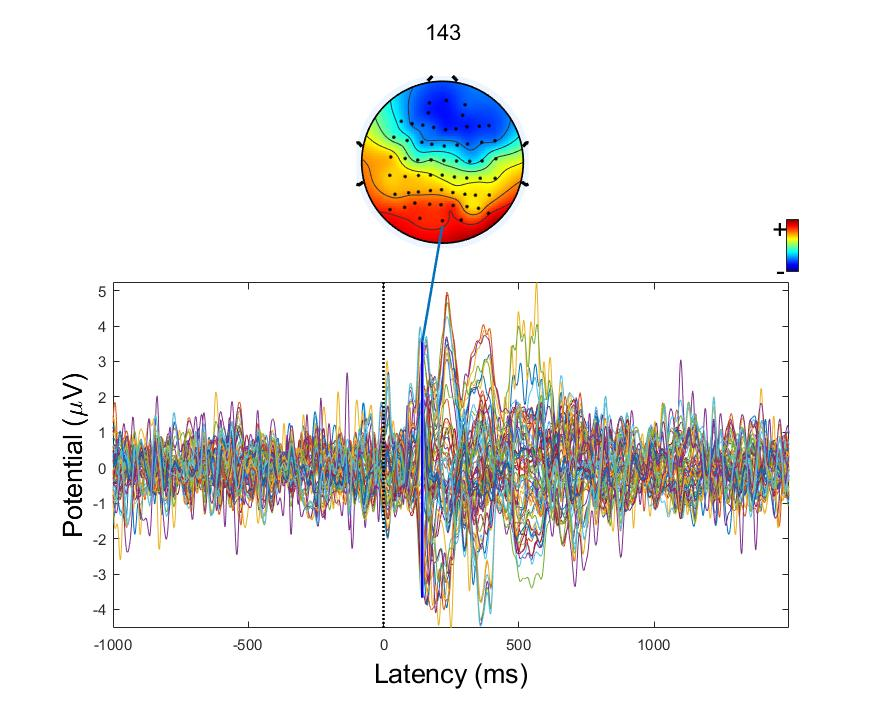
\includegraphics[scale=0.2]{listen_erp_11.jpg}}
	\caption{特征提取部分运行结果}\label{fig:feature}
\end{figure}

对标准刺激和偏差刺激的ERP进行对比,得到的结果如图(\ref{fig:ERPcompare})所示,点击不同的电极进行分析,我们发现,标准刺激在200$\sim$300ms之间达到峰值,而偏差刺激在500$\sim$600ms之间达到峰值,也就是说,偏差刺激得到的ERP峰值普遍比标准刺激得到的ERP峰值滞后300ms左右的时间。

\begin{figure}[htb]
\centering
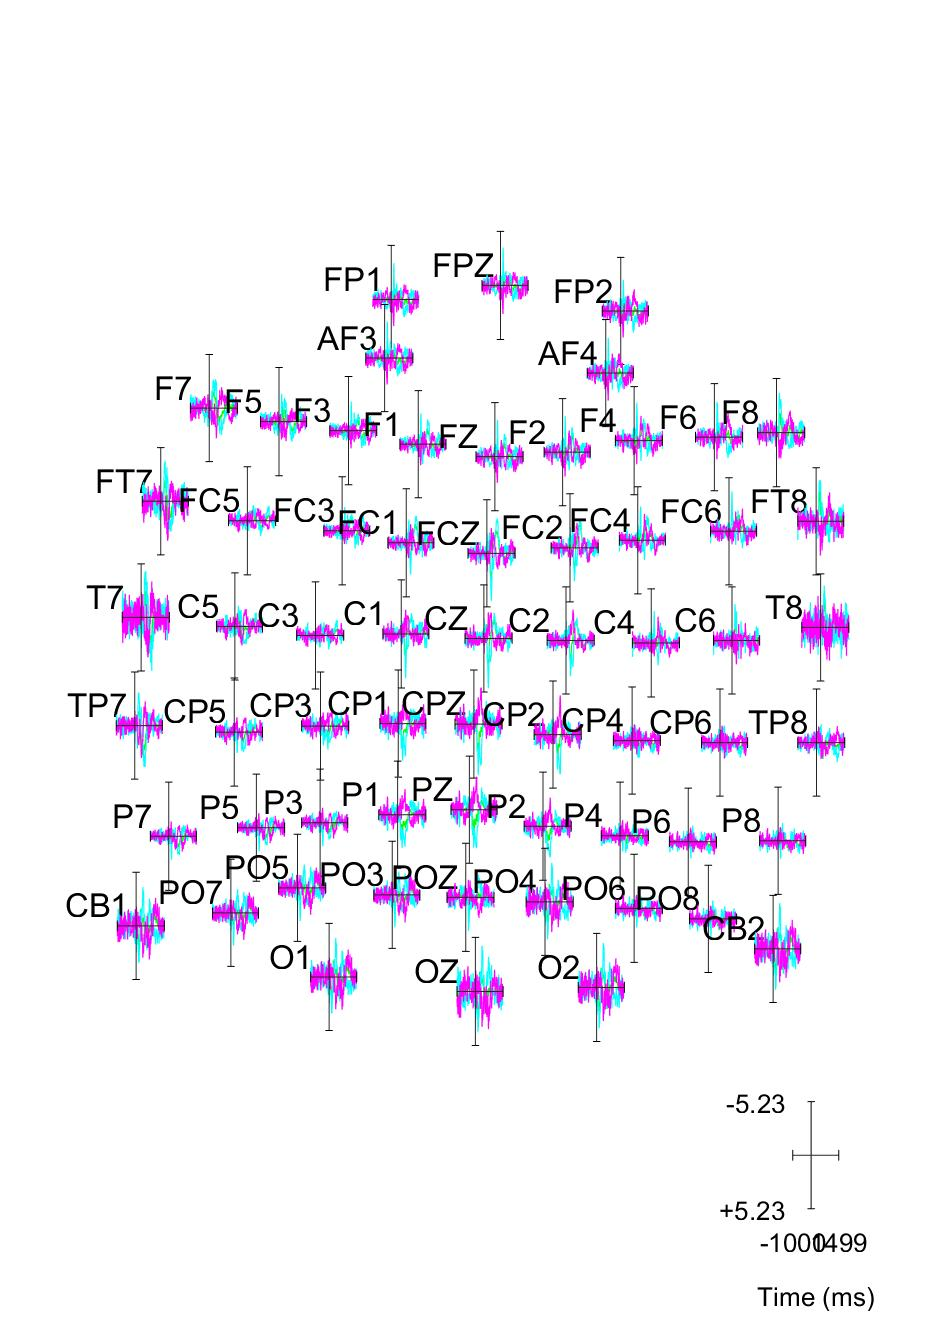
\includegraphics[height=0.4\textheight]{ERPcompare.jpg}
\caption{标准刺激与偏差刺激的ERP比较}\label{fig:ERPcompare}
\end{figure}

对偏差刺激进行分析,发现在565ms时达到波峰值,幅值约为5.0$\mu$V,主要活跃的脑区为左侧顶叶和左侧额叶,如图(\ref{fig:11high})所示,查看左侧额叶和左侧顶叶附近的电极,如图(\ref{fig:11highdetails})所示,在565ms左右也符合上述变化趋势,特别是电极FT7(\ref{fig:FT7high})、T7(\ref{fig:T7high})、C5(\ref{fig:C5high})、TP7(\ref{fig:TP7high})的特征很明显。

对标准刺激进行分析,发现在450ms时达到波峰值,幅值约为3.5$\mu$V,主要活跃的脑区为左侧顶叶和左侧额叶,如图(\ref{fig:22low})所示,查看左侧额叶和左侧顶叶附近的电极,如图(\ref{fig:22lowdetails})所示,在450ms左右也符合上述变化趋势,特别是电极FT7(\ref{fig:FT7low})、T7(\ref{fig:T7low})、C5(\ref{fig:C5low})、TP7(\ref{fig:TP7low})、P7(\ref{fig:P7low})的特征很明显。

\begin{figure}[htb]
\centering
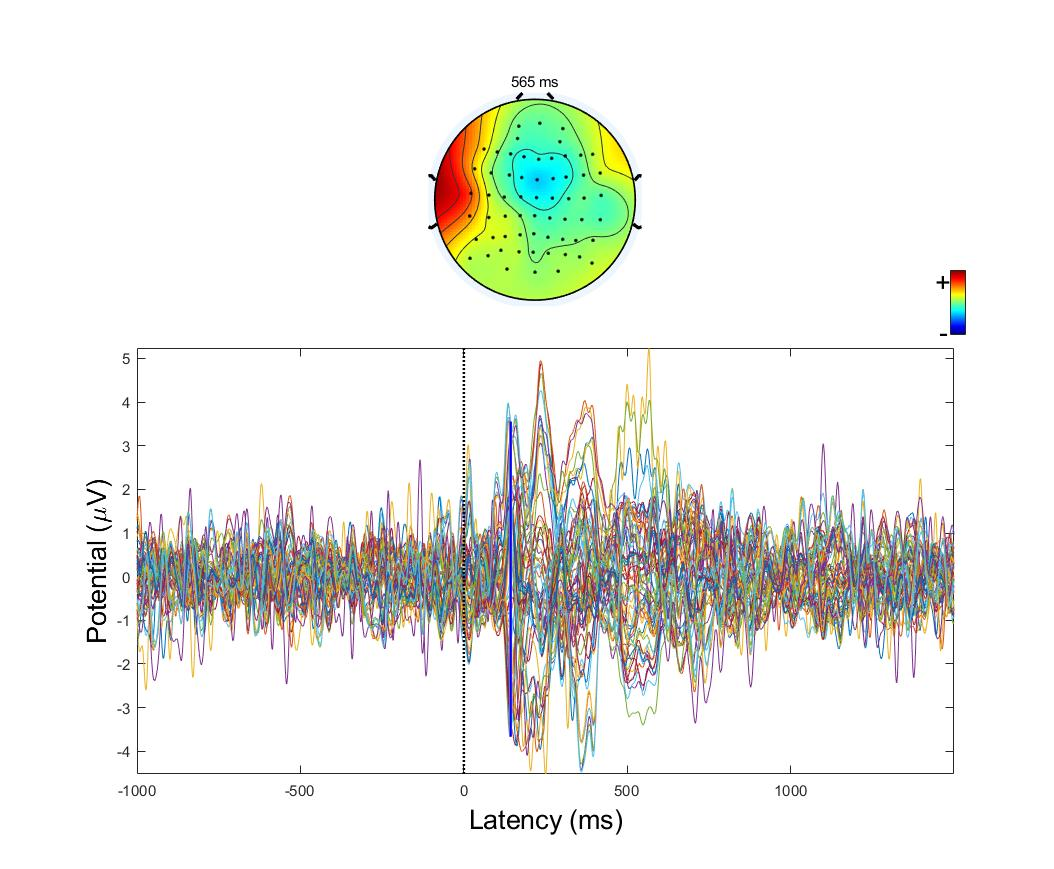
\includegraphics[scale=0.4]{11high.jpg}
\caption{偏差刺激的峰值}\label{fig:11high}
\end{figure}

\begin{figure}[htb]
\centering
	\subfloat[F7电极对偏差刺激的ERP]{
		\label{fig:F7high}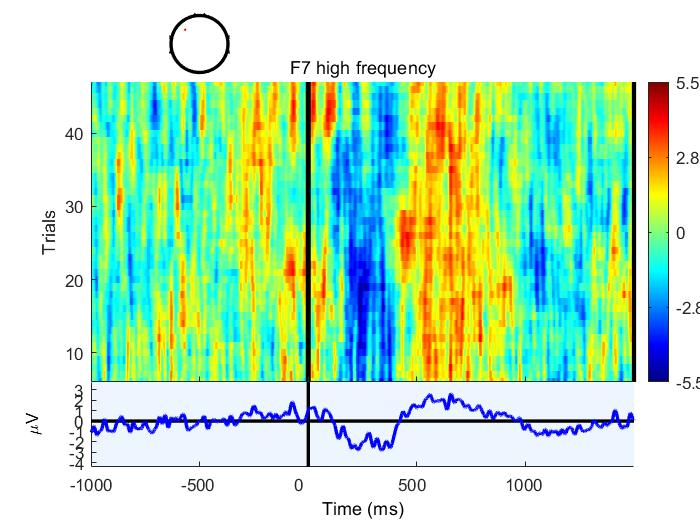
\includegraphics[width=.25\textwidth]{F7high.jpg}}
	\subfloat[F5电极对偏差刺激的ERP]{
		\label{fig:F5high}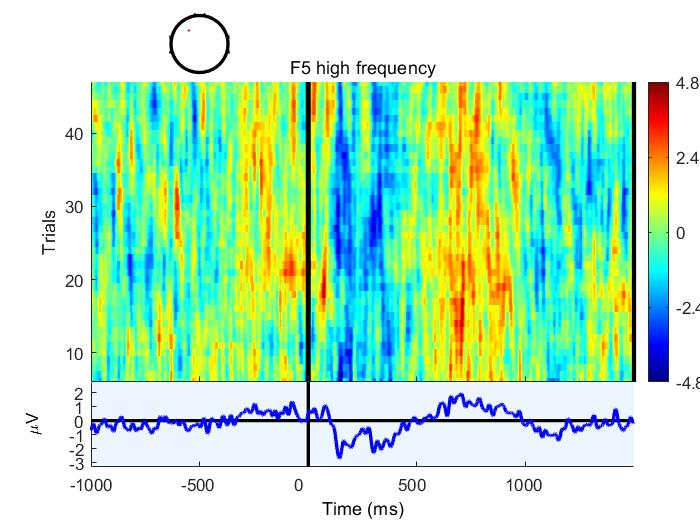
\includegraphics[width=.25\textwidth]{F5high.jpg}}
	\subfloat[FT7电极对偏差刺激的ERP]{
		\label{fig:FT7high}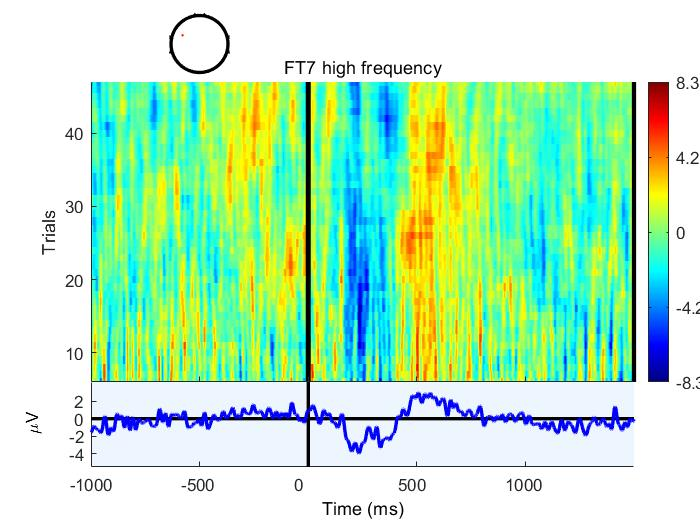
\includegraphics[width=.25\textwidth]{FT7high.jpg}}
	\subfloat[FC5电极对偏差刺激的ERP]{
		\label{fig:FC5high}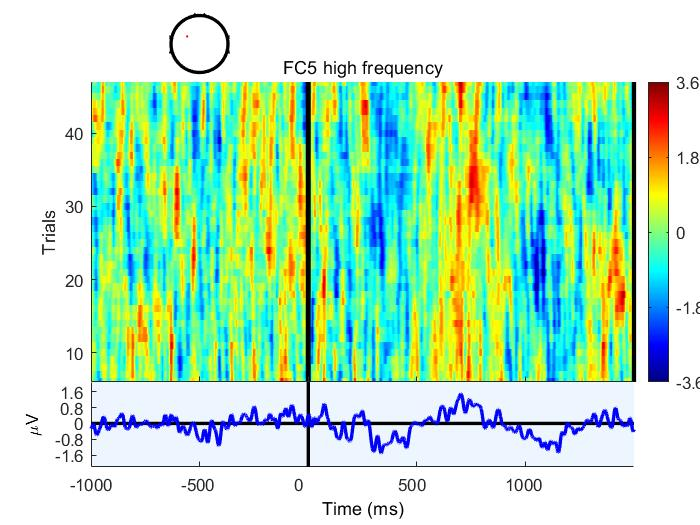
\includegraphics[width=.25\textwidth]{FC5high.jpg}}
	\\
	\subfloat[FC3电极对偏差刺激的ERP]{
		\label{fig:FC3high}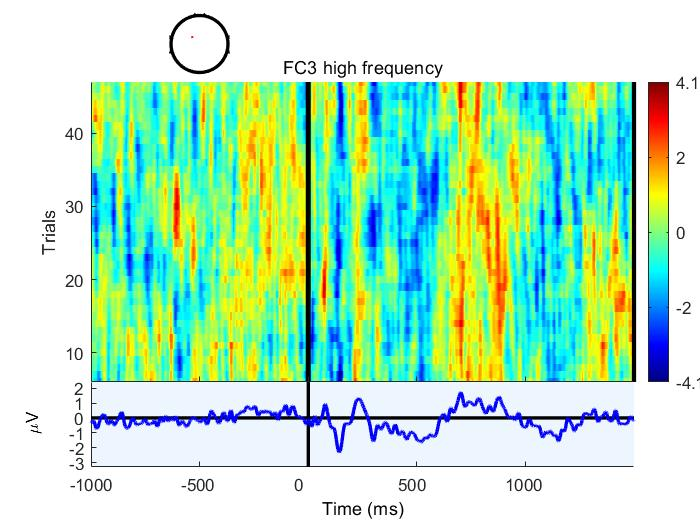
\includegraphics[width=.25\textwidth]{FC3high.jpg}}
	\subfloat[T7电极对偏差刺激的ERP]{
		\label{fig:T7high}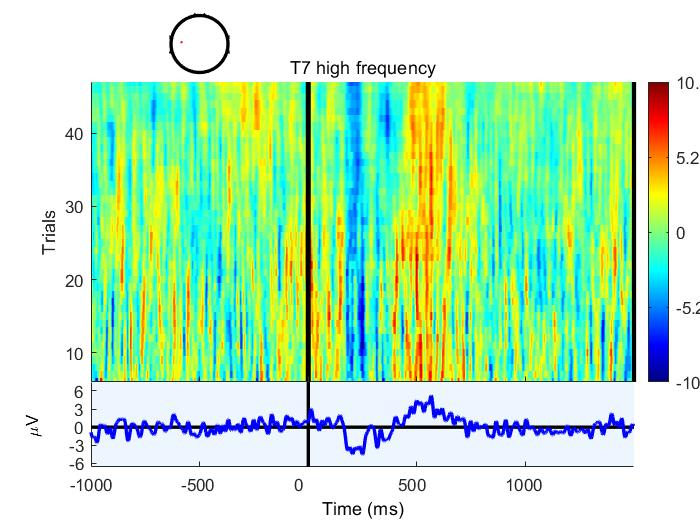
\includegraphics[width=.25\textwidth]{T7high.jpg}}
	\subfloat[C5电极对偏差刺激的ERP]{
		\label{fig:C5high}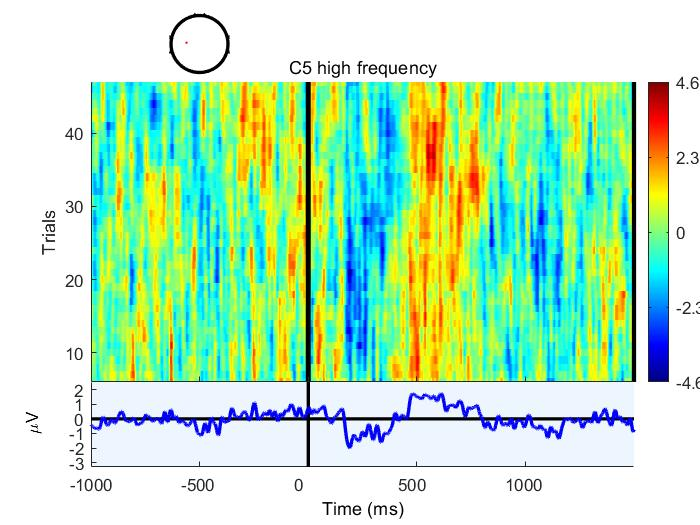
\includegraphics[width=.25\textwidth]{C5high.jpg}}
	\subfloat[C3电极对偏差刺激的ERP]{
		\label{fig:C3high}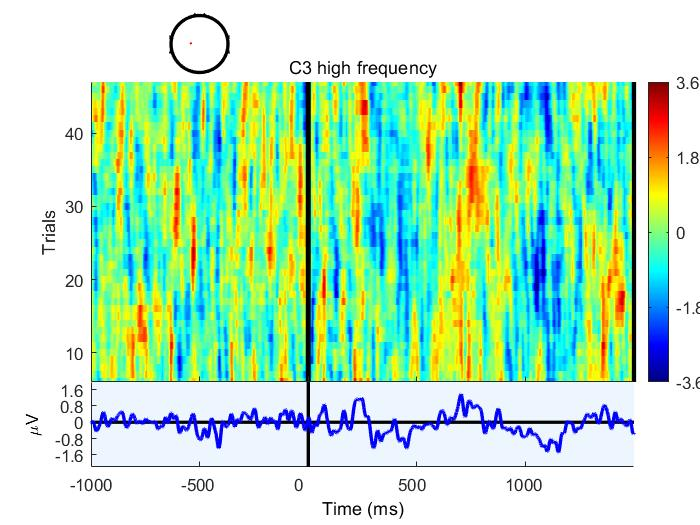
\includegraphics[width=.25\textwidth]{C3high.jpg}}
	\\
	\subfloat[TP7电极对偏差刺激的ERP]{
		\label{fig:TP7high}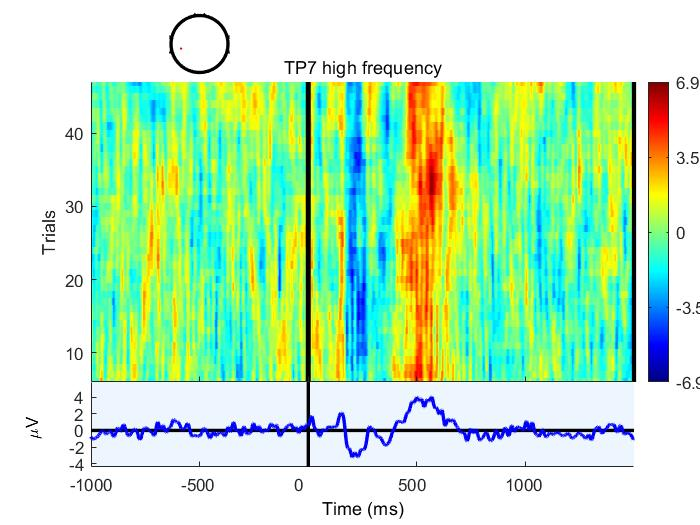
\includegraphics[width=.25\textwidth]{TP7high.jpg}}
	\subfloat[CP3电极对偏差刺激的ERP]{
		\label{fig:CP3high}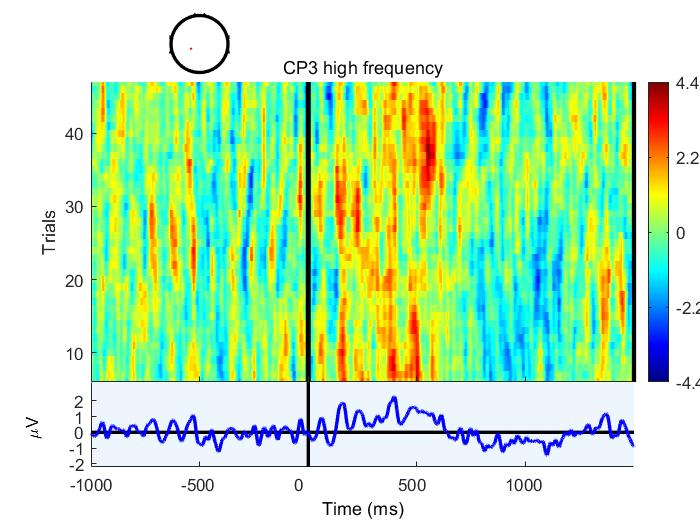
\includegraphics[width=.25\textwidth]{CP3high.jpg}}
	\subfloat[P7电极对偏差刺激的ERP]{
		\label{fig:P7high}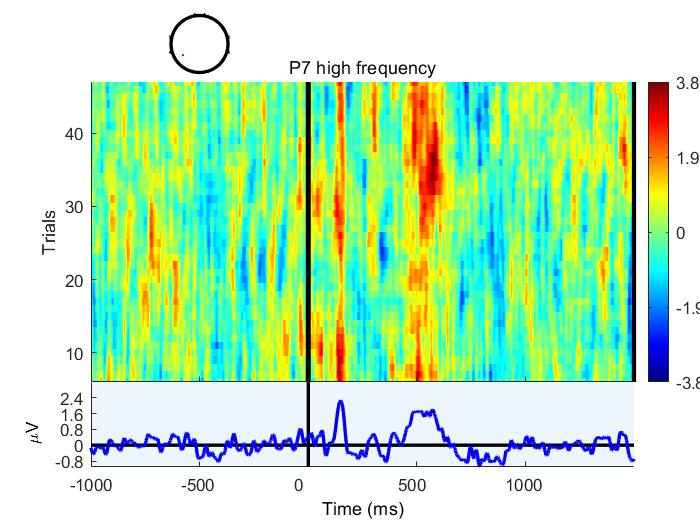
\includegraphics[width=.25\textwidth]{P7high.jpg}}
	\subfloat[P5电极对偏差刺激的ERP]{
		\label{fig:P5high}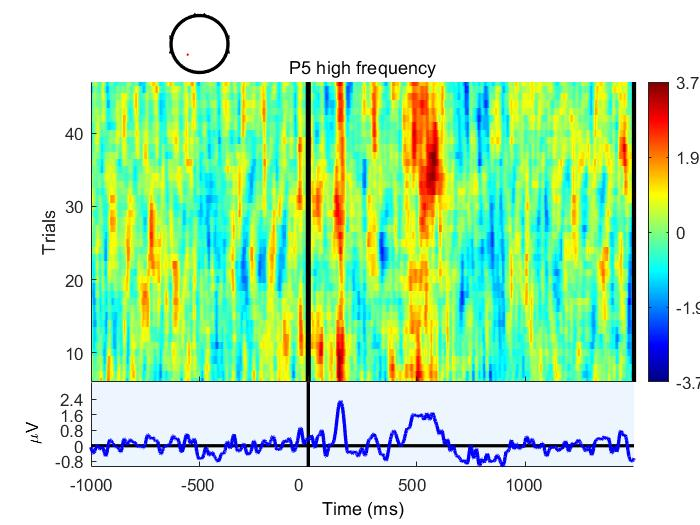
\includegraphics[width=.25\textwidth]{P5high.jpg}}
\caption{左侧额叶的左侧顶叶附近电极对偏差刺激的ERP}\label{fig:11highdetails}
\end{figure}

\begin{figure}[htb]
\centering
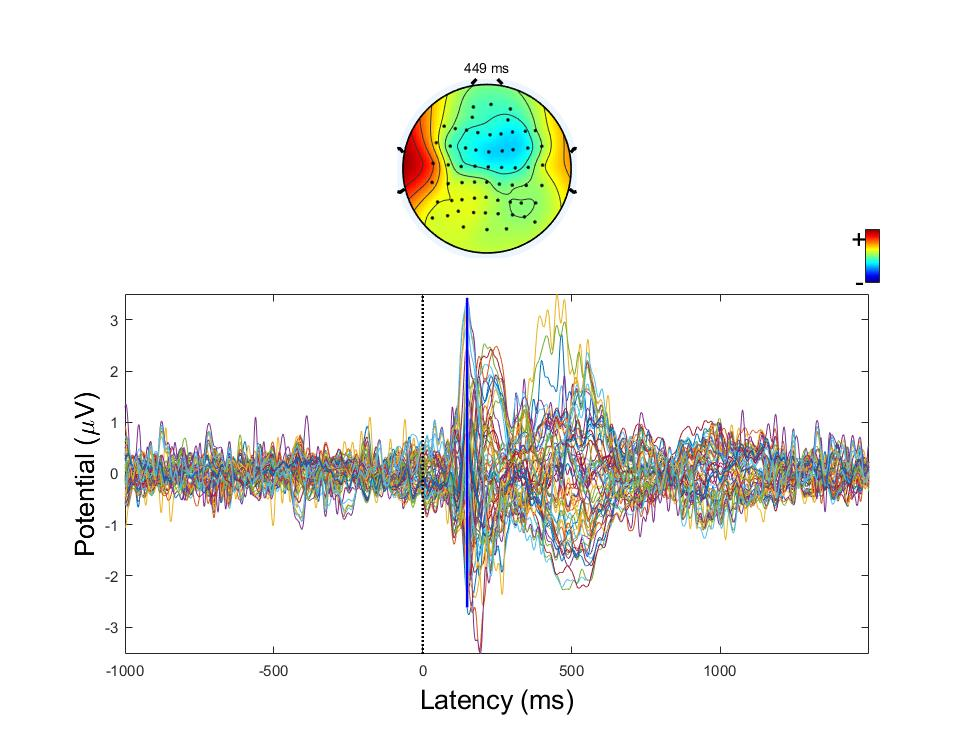
\includegraphics[scale=0.4]{22low.jpg}
\caption{标准刺激的峰值}\label{fig:22low}
\end{figure}

\begin{figure}[htb]
\centering
	\subfloat[F7电极对标准刺激的ERP]{
		\label{fig:F7low}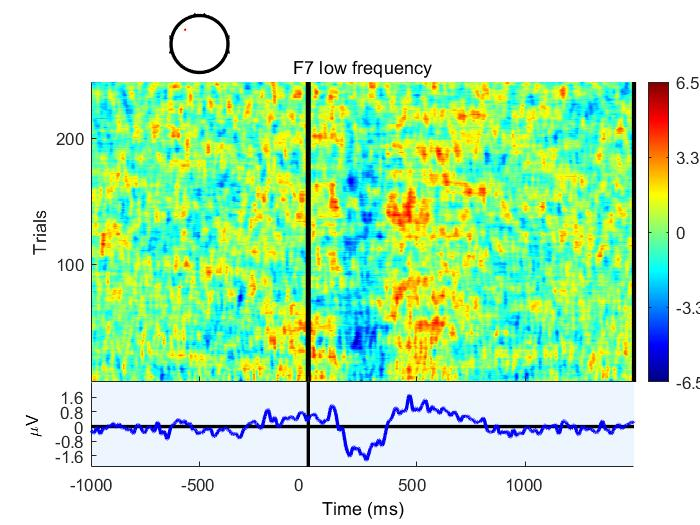
\includegraphics[width=.25\textwidth]{F7low.jpg}}
	\subfloat[FT7电极对标准刺激的ERP]{
		\label{fig:FT7low}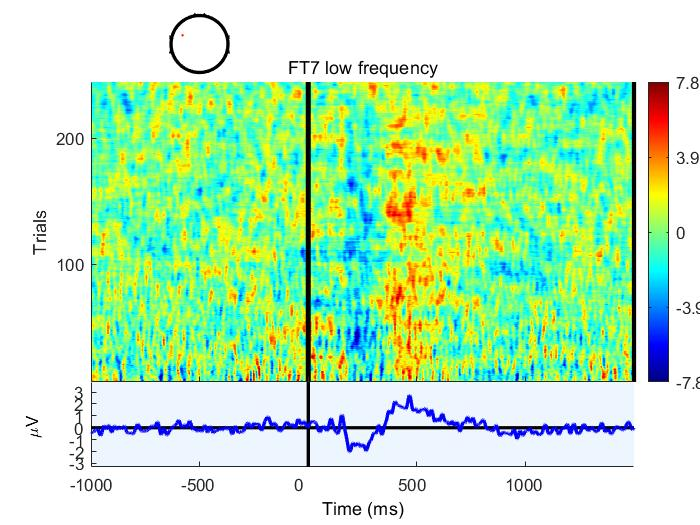
\includegraphics[width=.25\textwidth]{FT7low.jpg}}
	\subfloat[T7电极对标准刺激的ERP]{
		\label{fig:T7low}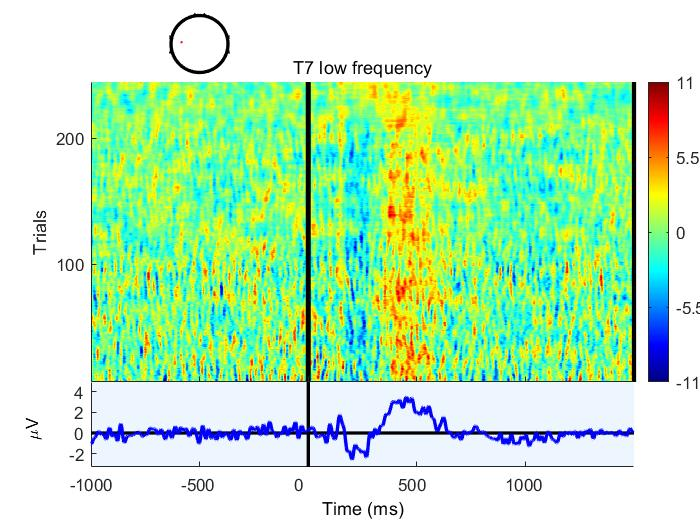
\includegraphics[width=.25\textwidth]{T7low.jpg}}
	\subfloat[C5电极对标准刺激的ERP]{
		\label{fig:C5low}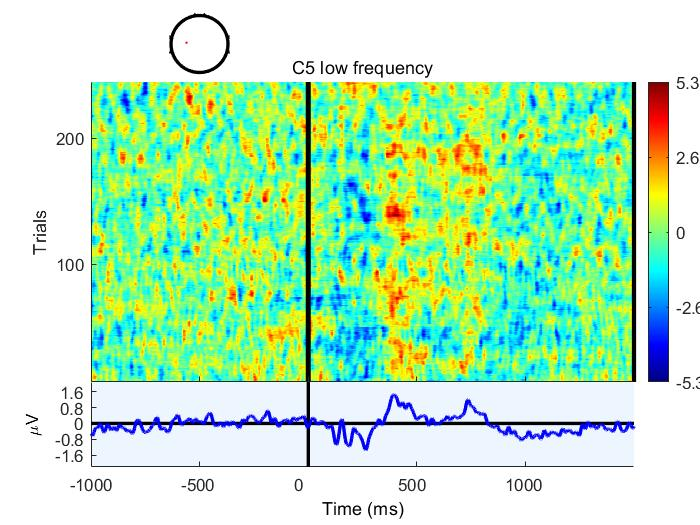
\includegraphics[width=.25\textwidth]{C5low.jpg}}
	\\
	\subfloat[TP7电极对标准刺激的ERP]{
		\label{fig:TP7low}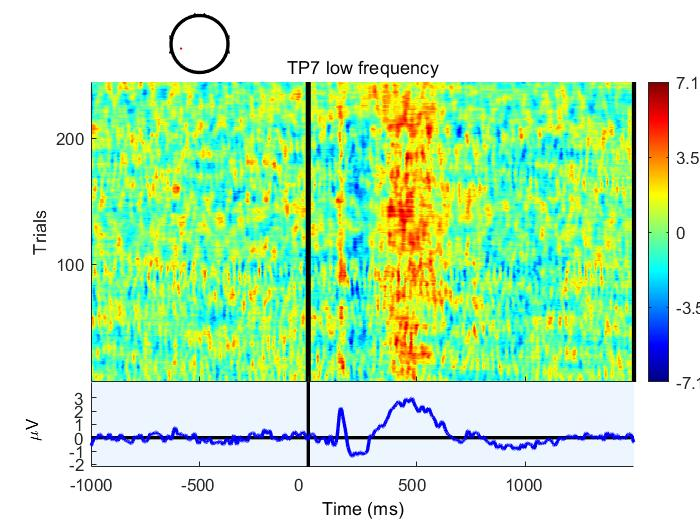
\includegraphics[width=.25\textwidth]{TP7low.jpg}}
	\subfloat[CP5电极对标准刺激的ERP]{
		\label{fig:CP5low}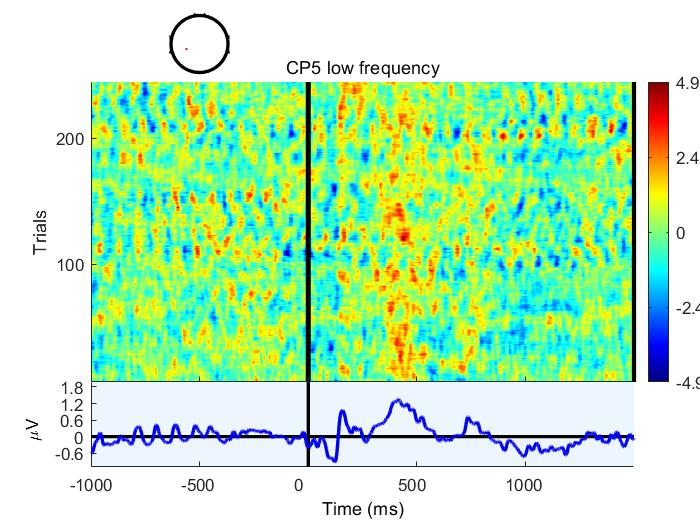
\includegraphics[width=.25\textwidth]{CP5low.jpg}}
	\subfloat[P7电极对标准刺激的ERP]{
		\label{fig:P7low}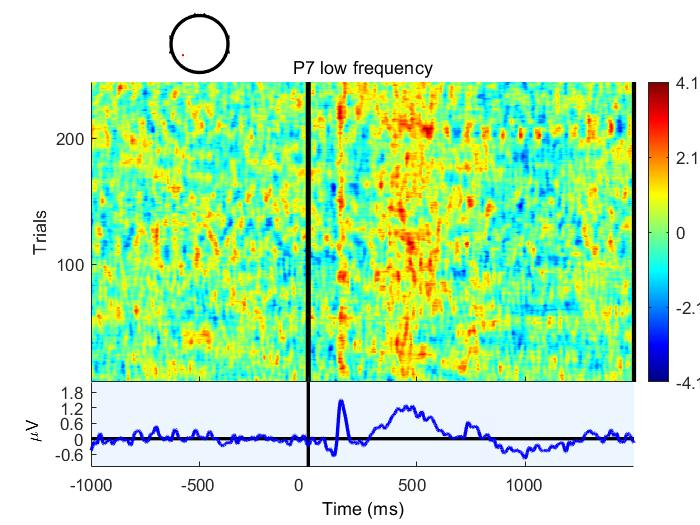
\includegraphics[width=.25\textwidth]{P7low.jpg}}
	\subfloat[P5电极对标准刺激的ERP]{
		\label{fig:P5low}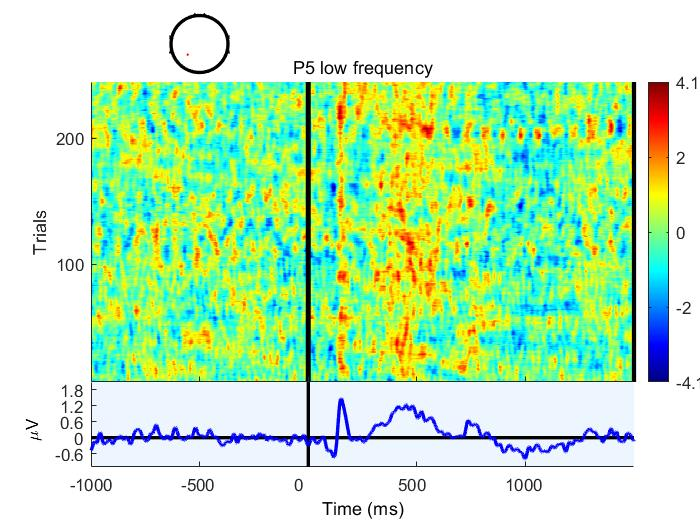
\includegraphics[width=.25\textwidth]{P5low.jpg}}
\caption{左侧额叶的左侧顶叶附近电极对标准刺激的ERP}\label{fig:22lowdetails}
\end{figure}


\paragraph{问题三}~{}

\begin{enumerate}
\item Event-related potentials in the auditory oddball as a function of EEG alpha phase at stimulus onset\cite{Barry2004}

\hspace{2em}本文旨在通过利用正交相位效应的概念,来研究固定时间间隔的听觉oddball实验中刺激作用时EEG的 $\alpha$波活动的情况与ERPs之间的关系。实验让14名受试者受到4组目标概率为50\%的150刺激,通过检查受试者对按钮按压的EEG的反应,对EEG信号进行滤波处理后,对每个受试者评估刺激前后的$\alpha$波。结果显示,在本次实验中,大脑状态对表现负向刺激的驱动力比正向刺激的驱动力高出8\%,且在waxing阶段会比waning阶段提高33\%,这与N1延迟增加和N2振幅减小相关。这些反映了刺激开始时$\alpha$波的频率和振幅的系统变化。因此,在固定时间间隔的的刺激范式中,动态调节EEG的成分频率,以便在刺激表现时更好地展示大脑状态,从而有差别地判断刺激过程在EEG结果中的相关性。

\item EEG alpha activity and the ERP to target stimuli in an auditory oddball paradigm\cite{Barry2000}

\hspace{2em}本文采用了固定时间间隔刺激的oddball实验,以获得ERP中N1P2和N2P3组件的峰-峰幅度与受试者体内受刺激前$\alpha$活性水平的关系。实验采取两种不同的音调作为刺激,概率各为50\%,分别向14位受试者提供了600个听觉刺激,需要受试者按目标按钮对不同音调做区分。对于每个试验,通过从8到13 Hz的滤波来评估Pz刺激前的$\alpha$活性,并使用$\alpha$波的RMS幅度对Pz和Cz处的ERPs进行排序。 对Pz和Cz处的分量振幅与Pz处的刺激前$\alpha$波建立关系,发现刺激前潜伏期的自发性脑电图与刺激后的$\alpha$波峰和波谷强烈相关。实验结果证实了中枢神经系统激活与刺激导致ERP的变化之间存在密切的关系。

\item Principal components analysis of Laplacian waveforms as a generic method for identifying ERP generator patterns: I. Evaluation with auditory oddball tasks\cite{Kayser2006}

\hspace{2em}本文评估了基于PCA的ERP波形简化与无参考Laplacian变换的有效性和可比性,以分离听觉oddball实验中与任务和响应相关的ERP生成器模式。实验中记录了66位惯用右手的成年人在使用音节或音调进行奇数球测试时记录的鼻子参考ERP,并计算球形样条电流源密度(CSD)波形以锐化ERP头皮形貌并消除体积传导的影响。ERP和CSD数据作为基于协方差的不受限制的时间PCA模型的输入,以分离时间和空间上存在相关性的ERP和CSD。

\hspace{2em}实验结果显示,相应刺激的ERP和CSD结果与已知的ERP成分相关。例如,可以从包围Sylvian裂缝的前槽和后源中中央的N1的偶极组织附近明显看到。与N2相关的因素以不对称的额外侧(音调:额颞R>L)和顶颞(语音:顶颞L>R)汇为特征。一个单一的ERP因子总结了顶叶P3的活性,以及前叶的阴性反应。相反,两个CSD因子在360ms和560ms达到峰值,将具有前汇的顶叶P3源与具有明显局限性Fz汇的中心顶叶P3源区分开来。与按按钮相比,静默计数的顶叶较小,但左侧颞叶P3源较大。

\hspace{2em}实验结果表明,CSD变换是ERP数据PCA的一个有价值的预处理步骤,为普遍存在的参考问题提供了一个独特的、有意义的解决方案。通过减少ERP冗余和生成更清晰、更简单的脑地形图,并且不丢失或扭曲任何感兴趣的效果,CSD-PCA解决方案复刻并扩展了以前与任务和响应相关的发现。

\item ERP measures of stimulus processing during an auditory oddball task in Parkinson's disease: Evidence for an early information processing deficit\cite{Wright1996}

\hspace{2em}本文将17名非特发性帕金森氏病的非痴呆患者与年龄和性别相匹配的对照组进行听觉oddball任务比较。通过无声计数或按下按钮来响应低概率目标音调。帕金森组的N1振幅减弱至目标音和非目标音,表明早期信息处理受到损害。相反,P2、N2和P3的幅度并未将患者与对照区分开。计数目标时,帕金森组几个峰值潜伏期(P2,N2和P3)增加,而通过按按钮确定目标时,只有N2被延迟。N2潜伏期越长,表明刺激分类所需的时间增加。早期ERP成分的幅度和潜伏期变化为帕金森氏病的早期信息处理受损提供了证据。

\item Auditory processing in an inter-modal oddball task: Effects of a combined auditory/visual standard on auditory target ERPs\cite{Brown2007}

\hspace{2em}先前的研究在多模式联动任务中对听觉oddball实验的受试者的ERP进行的研究表明,早期成分受模式内过程的影响,而ERP后期的成分(大约200$\sim$400ms)受多模式和多模式的影响。由此得出的结论是,听觉目标处理存在不同的阶段,早期的特定于情态的阶段和较晚的取决于上下文的阶段。本文通过研究在异类游戏中同时呈现视觉标准刺激和听觉标准刺激,以确定在此任务中包括视觉标准刺激是否会影响ERP达到目标。听觉-视觉oddball任务包括定期提出的听觉和视觉标准刺激(80\%和不常见的听觉目标(20\%)。将听觉-视觉oddball任务中目标的ERP与具有相同听觉刺激且没有视觉标准的听觉oddball任务中的ERP进行了比较。结果表明,早期组件N100,P200和N200在任务之间没有区别。这与先前研究的结果一致,并证实了长达200ms的活动不受视觉标准刺激的影响。后来的P250,P300和P350组件较大,并且在听觉-视觉oddball任务中显示出较大的脑地形图差异。特别是,P300和P350成分被认为代表了独立的模态和模态内成分。总的来说,这项研究提供了听觉加工在早期情态依赖阶段和后期情境依赖阶段这两个阶段发生的进一步证据。


\end{enumerate}


\subsection{信息相关电位认知实验及结果分析}

\subsubsection{信息相关电位认知实验介绍}

\paragraph{实验目的及意义}~{}

当刺激材料含有信息时,脑在对刺激中的信息进行加工的过程中,是否会产生一系列信息加工相关的认知成分?信息加工过程中,脑活动的EEG/ERP表现是否存在?若存在,则该成分或者表现是否有一定的模式,呈现一定的规律?

\paragraph{实验流程}~{}

实验共有3轮,每轮5个blocks,每个block含有30个trials。
实验时长36min。
实验流程如图(\ref{fig:labinfor})所示
\begin{figure}[htb]
\centering
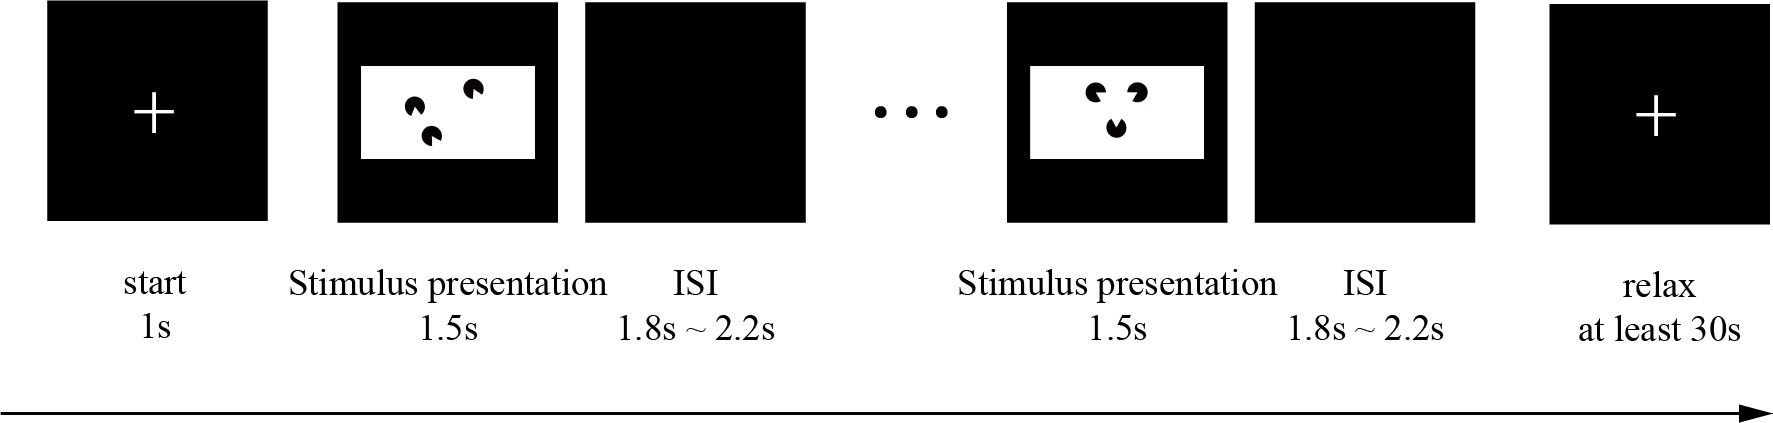
\includegraphics[scale=0.9]{infor.png}
\caption{信息相关电位认知实验流程图}\label{fig:labinfor}
\end{figure}

在每个trial中,被试需根据当前显示的图像是否含有信息进行判断,含有信息按下键盘方向键左键,不含有信息的按下键盘方向键右键。

\paragraph{问题}~{}

\begin{enumerate}
\item 请你分析在判断有信息和无信息时,准确率和反应时间有何区别?

准确率:
\begin{align}
\text{有信息刺激的准确率} = \frac{\text{有信息刺激时,判断为有的数量}}{\text{有信息刺激的数量}}\\
\text{无信息刺激的准确率} = \frac{\text{无信息刺激时,判断为无的数量}}{\text{无信息刺激的数量}}
\end{align}
反应时间为:在判断正确的trial中,反应时刻-刺激发生时刻

\item 请分析
\begin{enumerate}
\item 在有信息刺激时,花鸟图案刺激引起的ERP和几何图像刺激引起的ERP有何差异?
\item 在无信息刺激时,花鸟图案刺激引起的ERP和几何图像刺激引起的ERP有何差异?(分析ERP成分的幅值、潜伏期等差异即可)
\end{enumerate}

\item 请分析在几何图像trial中,含信息刺激引起的ERP与不含信息刺激引起的ERP有何差异?这些差异主要体现在哪些脑区(通过脑地形图说明)?
\end{enumerate}


\paragraph{信息相关电位实验事件码说明}~{}
\newline
31:三个扇形图案位置与开口方向完全随机分布,无信息刺激\\
32:三个扇形图案位置固定,开口方向固定,有信息刺激\\
33:三个扇形图案位置固定、开口方向随机,无信息刺激\\
41:四个扇形图案位置与开口方向完全随机分布,无信息刺激\\
42:四个扇形图案位置固定,开口方向固定,有信息刺激\\
43:四个扇形图案位置固定、开口方向随机,无信息刺激\\
51:花鸟图案完全随机分布,无信息刺激\\
52:花鸟图案能形成人脸轮廓,有信息刺激\\
53:花鸟图案完全随机分布,无信息刺激\\
1:判断为有信息刺激\\
2:判断为无信息刺激

\subsubsection{信息相关电位认知实验结果分析}

\paragraph{问题一}~{}

对实验数据进行预处理,得到采样频率为1000Hz的预处理实验数据,将EEG结构体的event属性导出到excel中,得到如图(\ref{fig:inforexcel})的结果。

\begin{figure}[htb]
\centering
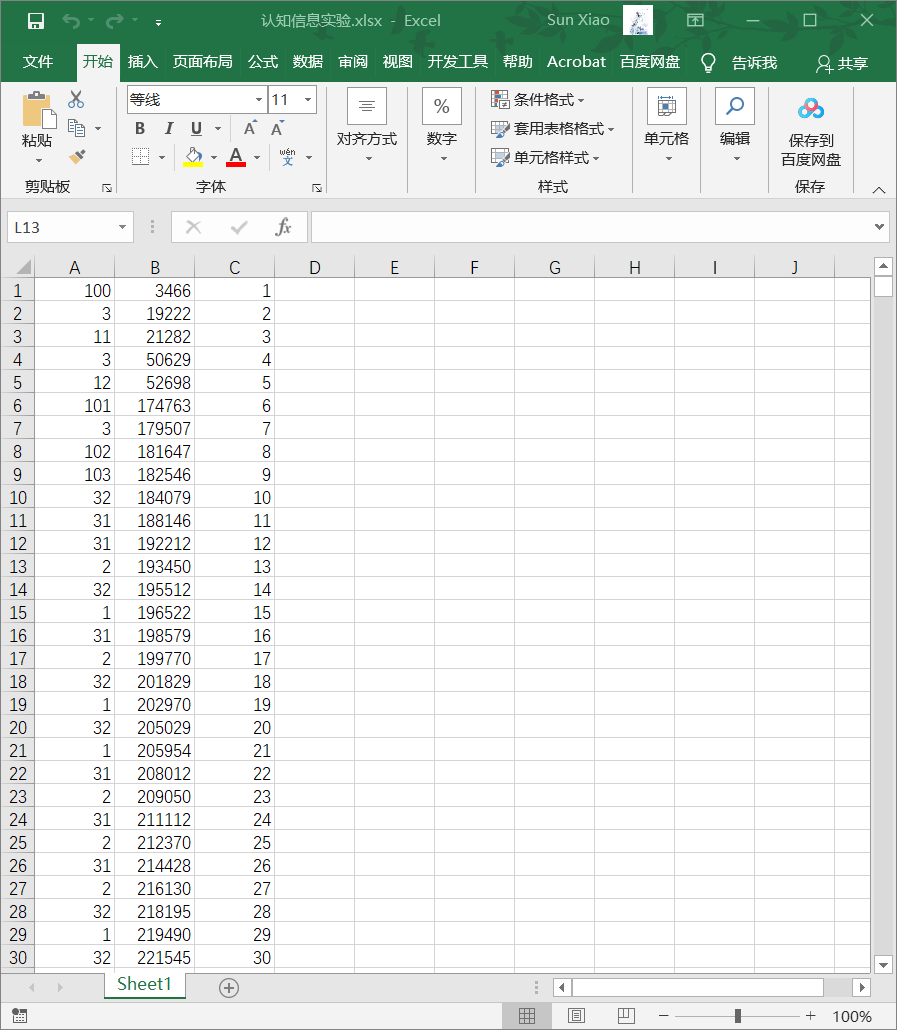
\includegraphics[scale=0.3]{inforexcel.png}
\caption{将信息相关电位实验的事件信息导入Excel结果}\label{fig:inforexcel}
\end{figure}

将Excel文件转化为csv文件,手动去掉了等待时间自己乱按的事件码,得到的data文件夹下的information.cv文件。编写代码计算事件码31、32、33、41、42、43、51、52和53对应的判断,并计算判断正确时的平均反应时长以及不同trial对应的有信息刺激准确率和无信息刺激准确率。

实验的代码见附录\ref{app:information}。

最终得到的结果如log文件所示。
\begin{lstlisting}[language=bash]
ineffective judge at line 2
ineffective judge at line 3
ineffective judge at line 63
ineffective judge at line 251
ineffective judge at line 254
ineffective judge at line 291
three sectors have information correct accuracy:0.9888888888888889
three sectors have no information correct accuracy:0.9888888888888889
the average of reaction time of three sectors is:946.1797752808989
four sectors have information correct accuracy:0.9888888888888889
four sectors have no information correct accuracy:1.0
the average of reaction time of four sectors is:942.9162011173185
flower and bird pattern have information correct accuracy:0.9333333333333333
flower and bird pattern have no information correct accuracy:1.0
the average of reaction time of flower and bird pattern is:958.0114942528736

\end{lstlisting}

根据结果来看,在实验中,我并没有出现对某个信息判断出错的情况,但是准确率并未达到100\%。这是因为每个trial刚开始的两三幅图片,系统并未等我作出判断就进行了翻页,根据之后对于平均反应时间的测量,估计系统设置自动翻页的时间为1s,不知道是否为系统的bug,也希望这里改进一下,等待受试者作出判断后再翻页。

我将未及时进行判断的情况定义为失败的判断,因此得到:
\begin{enumerate}
\item 三个扇形图案有信息刺激准确率为98.89\%;
\item 三个扇形图案无信息刺激准确率为98.89\%;
\item 三个扇形图案的平均反应时间为946.18 ms;
\item 四个扇形图案有信息刺激准确率为98.89\%;
\item 四个扇形图案无信息刺激准确率为100\%;
\item 四个扇形图案的平均反应时间为942.92 ms;
\item 花鸟图案有信息刺激准确率为93.33\%;
\item 花鸟图案无信息刺激准确率为100\%;
\item 花鸟图案的平均反应时间为958.01 ms。
\end{enumerate}

从实验结果来看,对于四个扇形图案的有信息刺激判断准确率与三个图案的有信息刺激判断准确率持平,对于四个扇形图案的无信息刺激判断准确率较三个图案的无信息刺激判断准确率有所提升,但是平均反应时间几乎相同;花鸟图案的有信息刺激判断准确率有所下降,平均反应时间与扇形判断相比也更长,可能是由于实验时紧张,担心翻页过快而未来得及进行判断有关,从而导致的准确率下降。


\paragraph{问题二}~{}

此处几何图像的刺激以三个扇形的刺激为例。有信息刺激时,三个扇形图案刺激引起的ERP结果如图(\ref{fig:infor32})所示,选择100、200、300、400、500、600、700、800、900ms时的ERP叠加图像,如图(\ref{fig:infor32detail})所示,可以看到在刺激发生后的100$\sim$400ms内,主要活跃的脑区为右侧枕叶,在700$\sim$800ms之间,主要活跃的脑区为左侧额叶和左侧顶叶;花鸟图案刺激引起的ERP结果如图(\ref{fig:infor52})所示,选择100、200、300、400、500、600、700、800、900ms时的ERP叠加图像,如图(\ref{fig:infor52detail})所示,可以看到在刺激发生后的100$\sim$500ms内,主要活跃的脑区为右侧枕叶和部分左侧枕叶,在700ms左右主要活跃的脑区为左侧额叶。二者对比是的ERP图像如图(\ref{fig:infor3252})所示,选择右侧枕叶处的电极进行分析,右侧枕叶处相应电极的ERP叠加结果如图(\ref{fig:zhenye3252})所示,可以看到,在200ms左右,花鸟图案刺激下的右侧枕叶的ERP幅值要高于三个扇形图案引起的刺激,由此可以印证,右侧枕叶是对图像认知的能力较为活跃的区域。

\begin{figure}[htb]
\centering
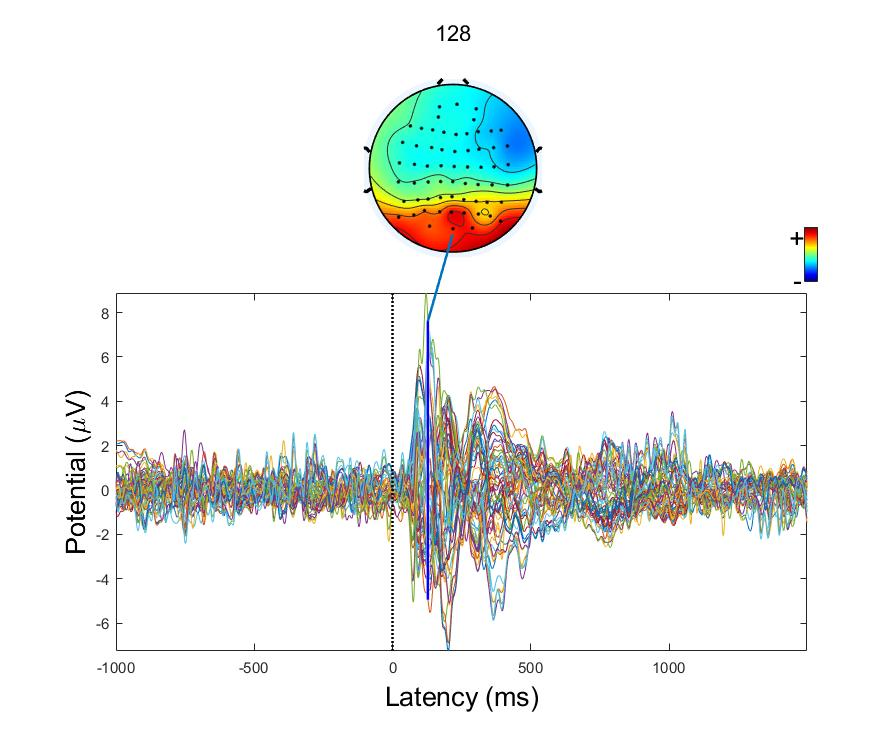
\includegraphics[scale=0.3]{infor32.jpg}
\caption{有信息刺激时,三个扇形图案刺激的ERP结果}\label{fig:infor32}
\end{figure}

\begin{figure}[htb]
\centering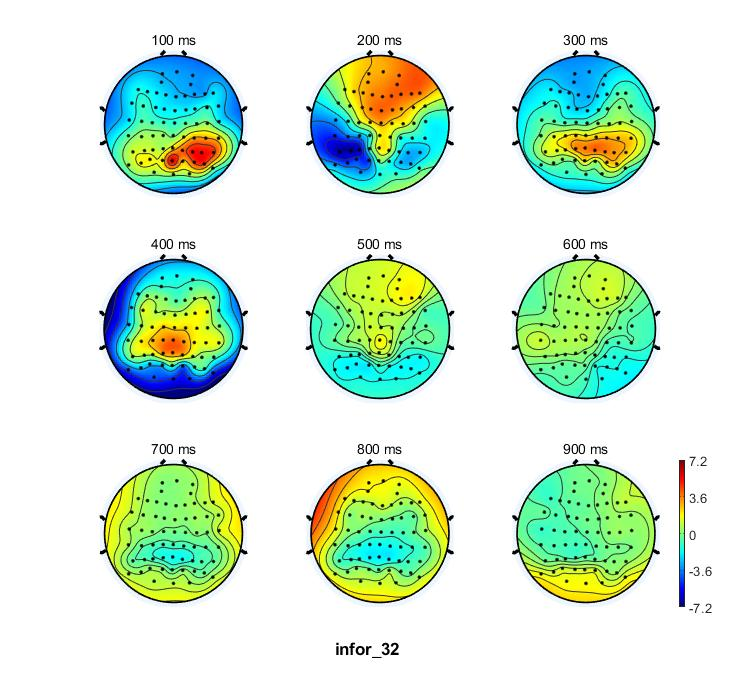
\includegraphics[scale=0.4]{infor32detail.jpg}
\caption{有信息刺激时,三个扇形图案刺激的ERP分时结果}\label{fig:infor32detail}
\end{figure}

\begin{figure}[htb]
\centering
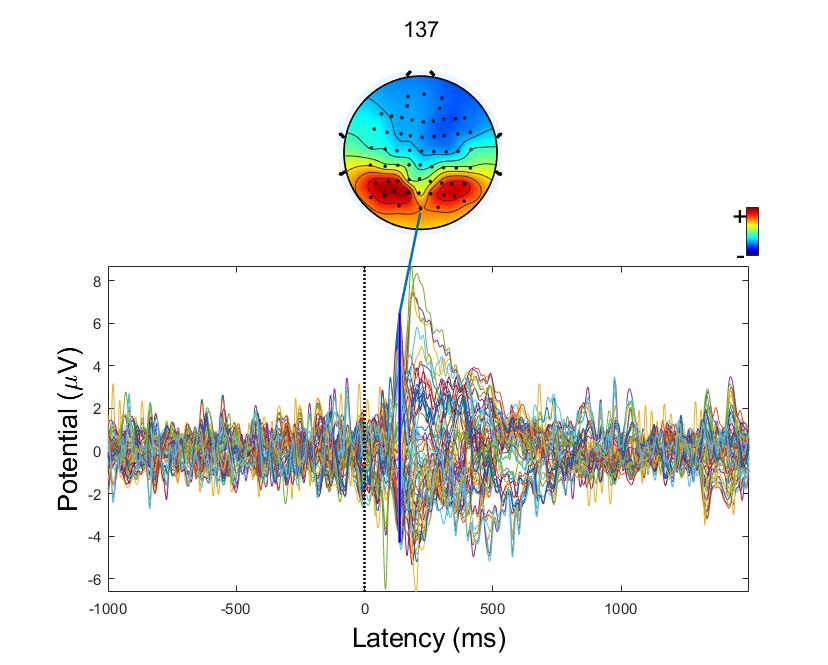
\includegraphics[scale=0.3]{infor52.jpg}
\caption{有信息刺激时,花鸟图案刺激的ERP结果}\label{fig:infor52}
\end{figure}

\begin{figure}[htb]
\centering
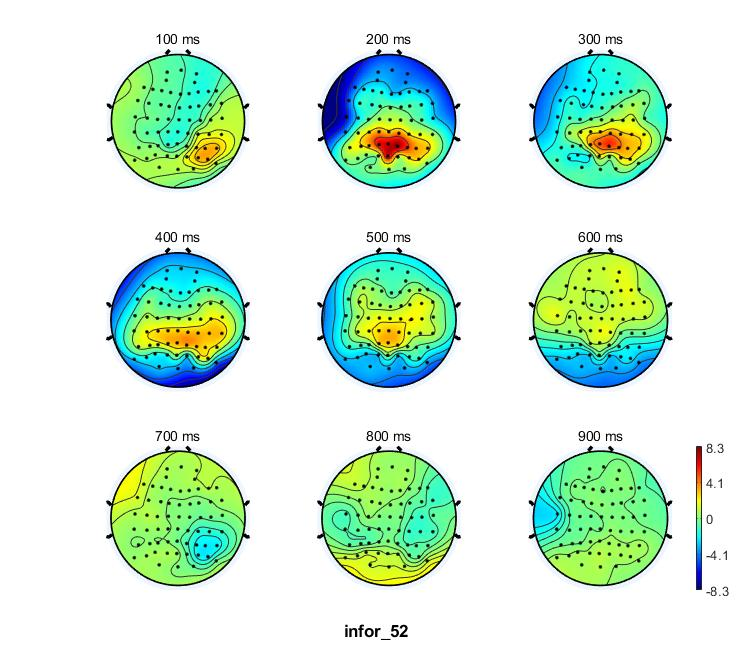
\includegraphics[scale=0.4]{infor52detail.jpg}
\caption{有信息刺激时,花鸟图案刺激的ERP分时结果}\label{fig:infor52detail}
\end{figure}

\begin{figure}[htb]
\centering
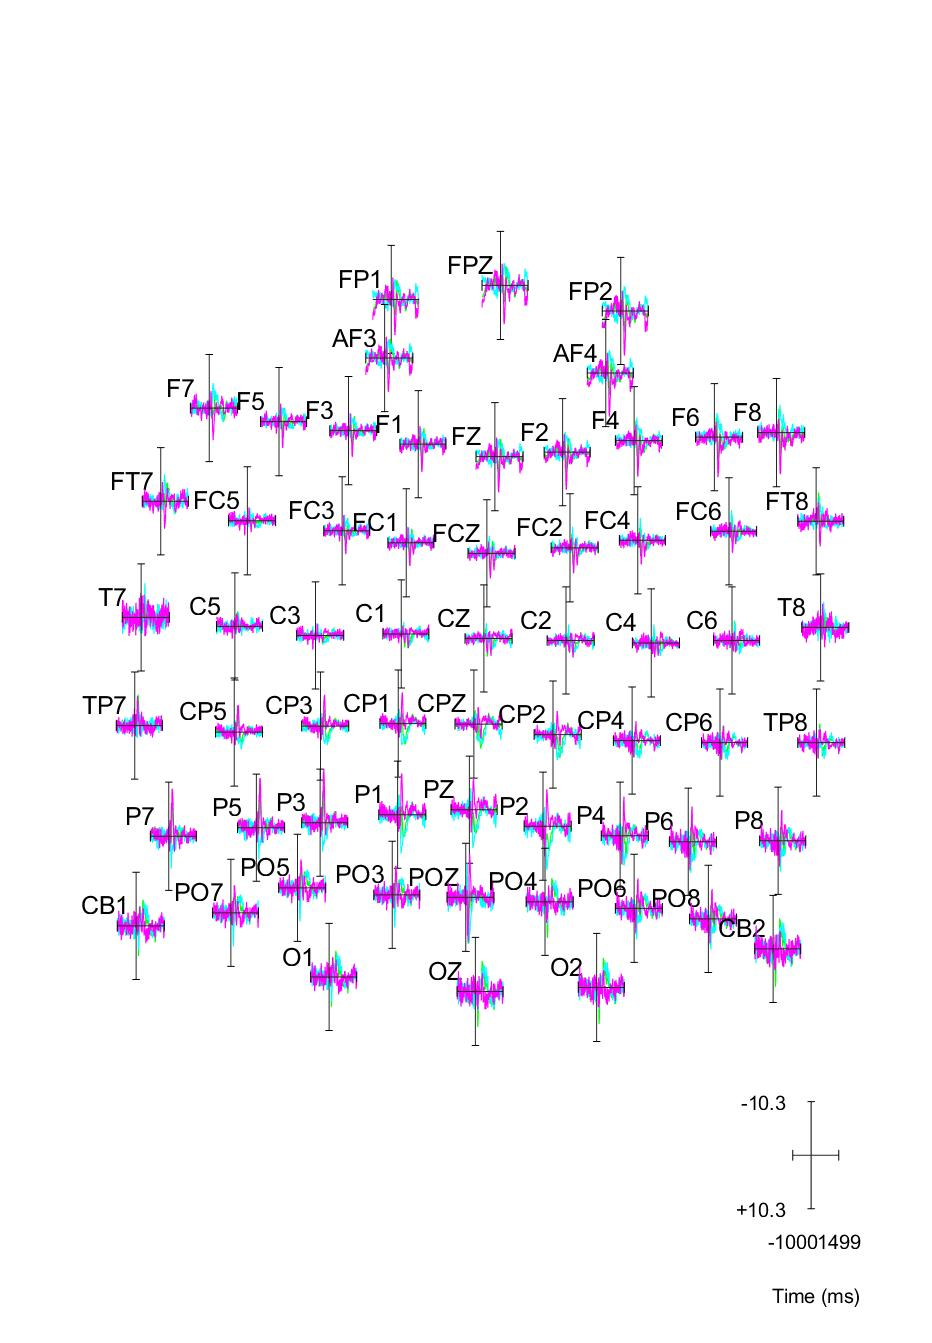
\includegraphics[height=0.4\textheight]{infor3252.jpg}
\caption{有信息刺激时,三个扇形图案刺激与花鸟图案刺激的ERP比较}\label{fig:infor3252}
\end{figure}

\begin{figure}[htb]
\centering
	\subfloat[CP1电极几何图形和花鸟图案ERP对比]{
		\label{fig:CP13252}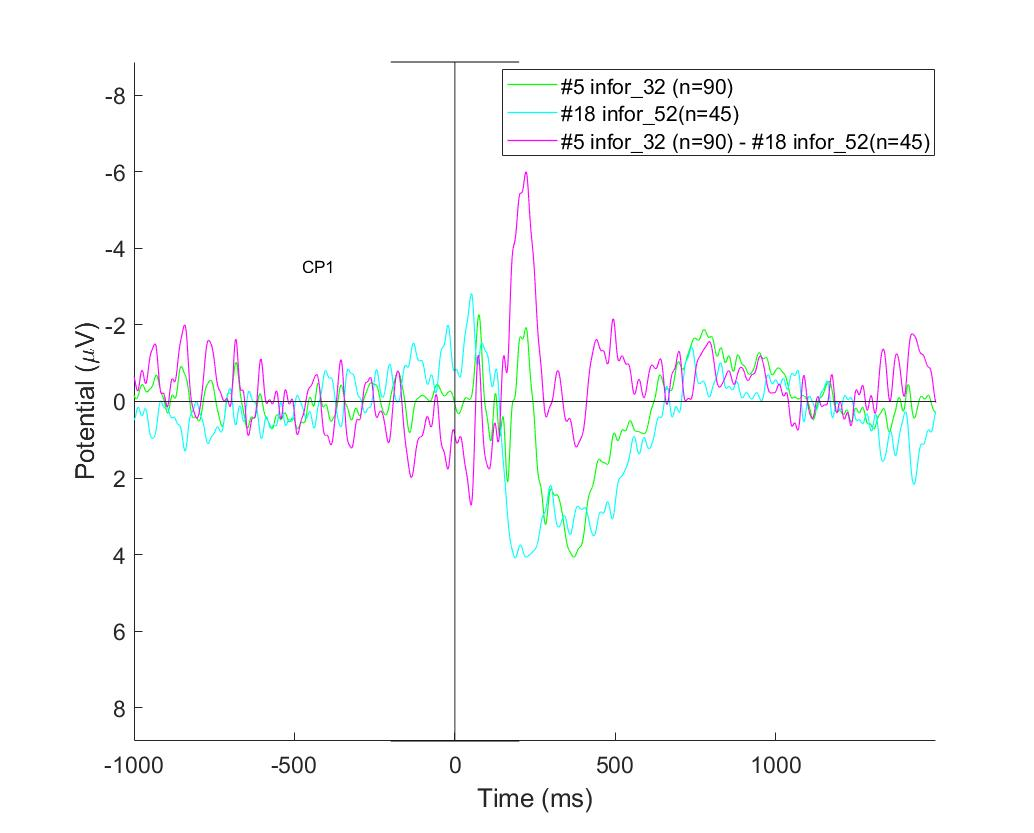
\includegraphics[width=.33\textwidth]{CP13252.jpg}}
	\subfloat[CPZ电极几何图形和花鸟图案ERP对比]{
		\label{fig:CPZ3252}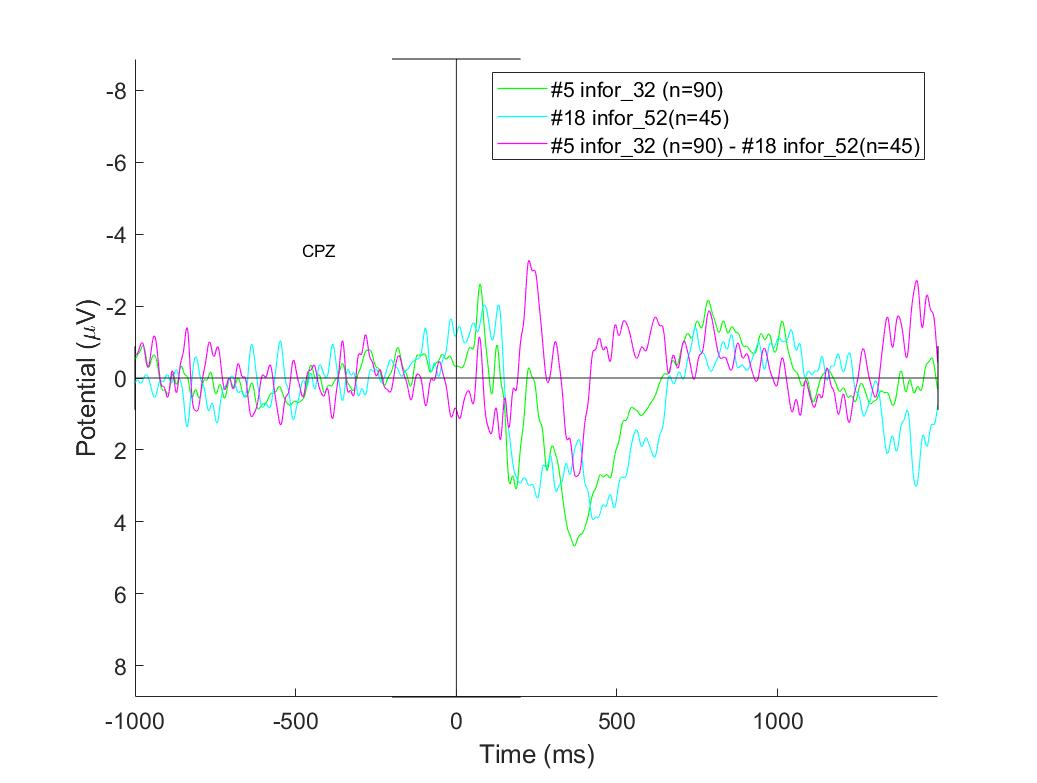
\includegraphics[width=.33\textwidth]{CPZ3252.jpg}}
	\subfloat[CP2电极几何图形和花鸟图案ERP对比]{
		\label{fig:CP23252}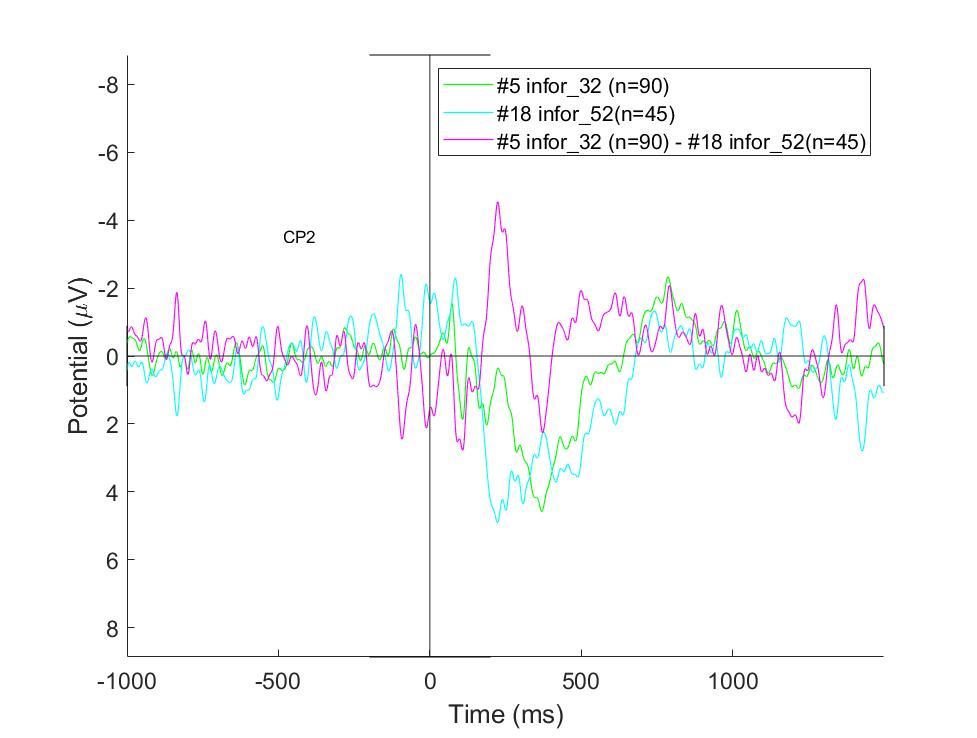
\includegraphics[width=.33\textwidth]{CP23252.jpg}}
	\\
	\subfloat[CP4几何图形和花鸟图案ERP对比]{
		\label{fig:CP43252}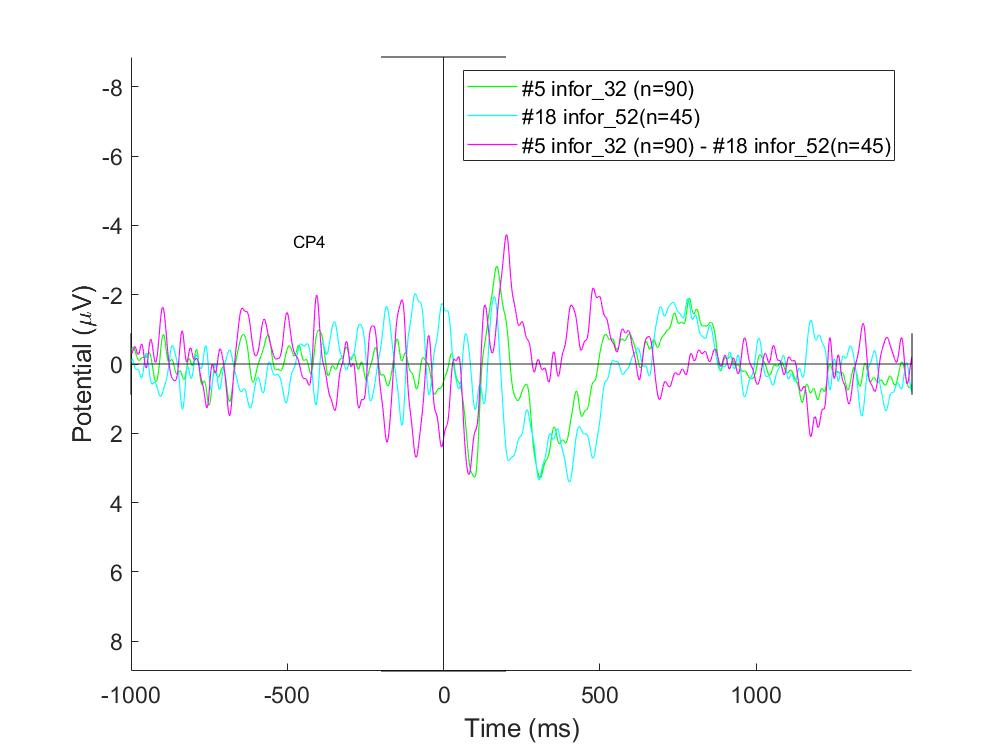
\includegraphics[width=.33\textwidth]{CP43252.jpg}}
	\subfloat[P1几何图形和花鸟图案ERP对比]{
		\label{fig:P13252}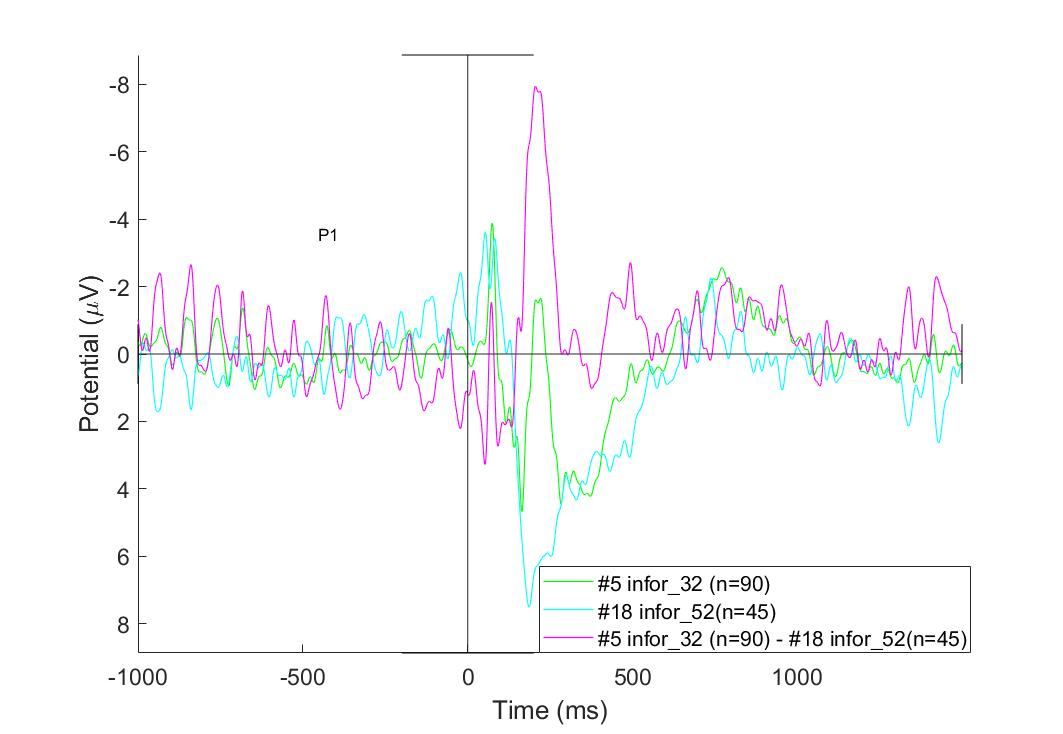
\includegraphics[width=.33\textwidth]{P13252.jpg}}
	\subfloat[PZ几何图形和花鸟图案ERP对比]{
		\label{fig:PZ3252}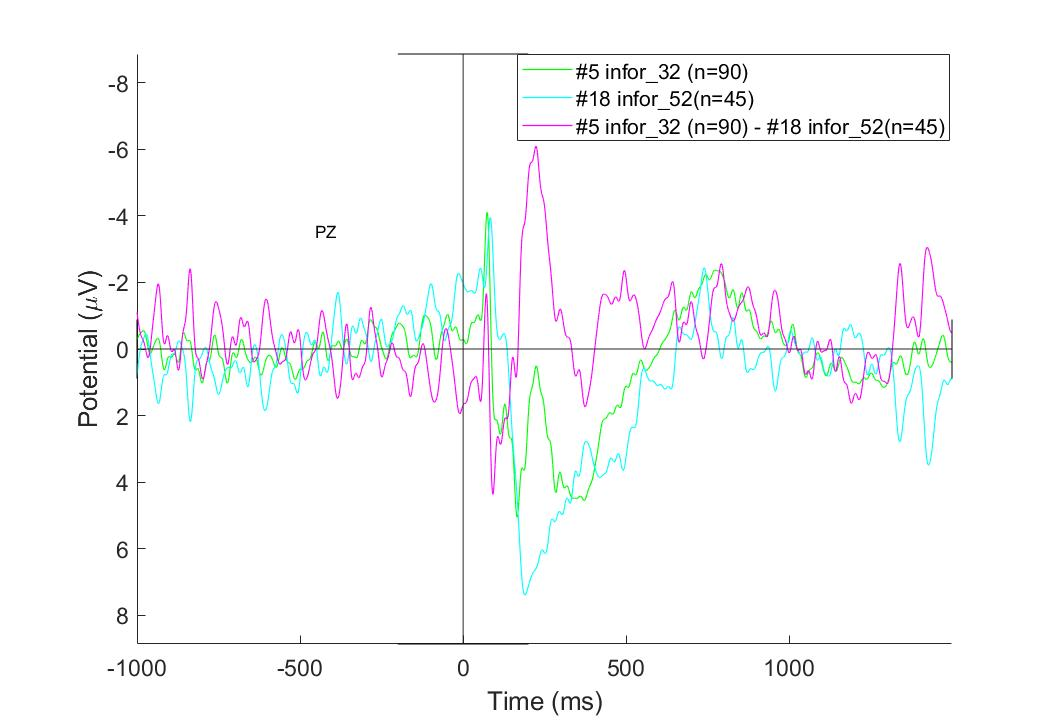
\includegraphics[width=.33\textwidth]{PZ3252.jpg}}
	\\
	\subfloat[P2几何图形和花鸟图案ERP对比]{
		\label{fig:P23252}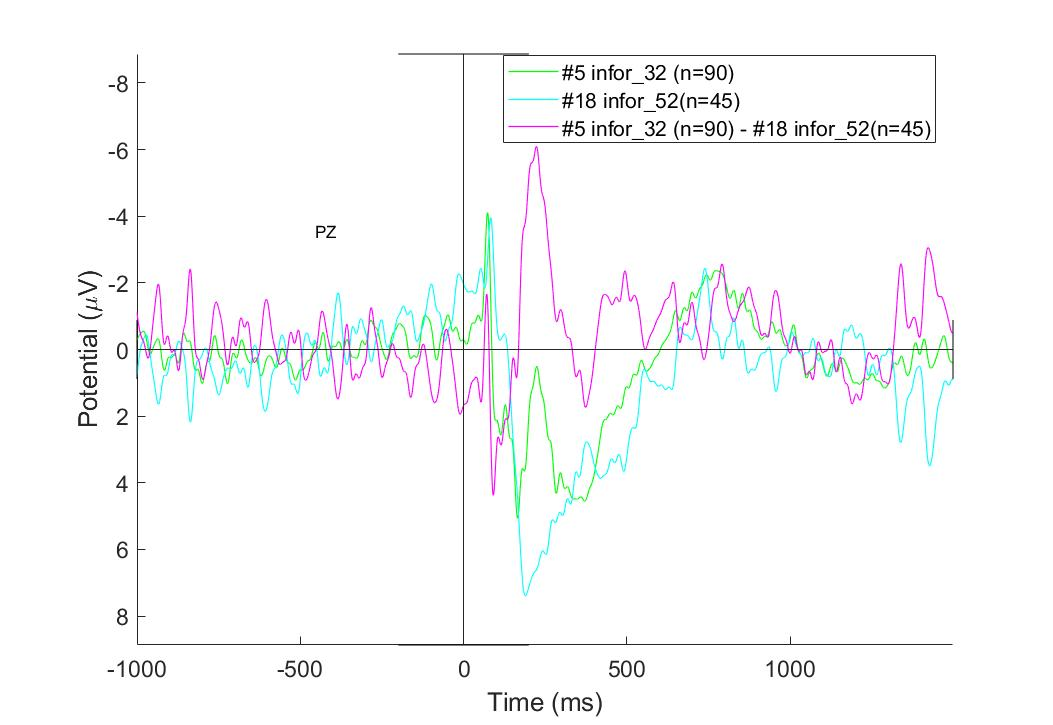
\includegraphics[width=.33\textwidth]{P23252.jpg}}
	\subfloat[P4几何图形和花鸟图案ERP对比]{
		\label{fig:P43252}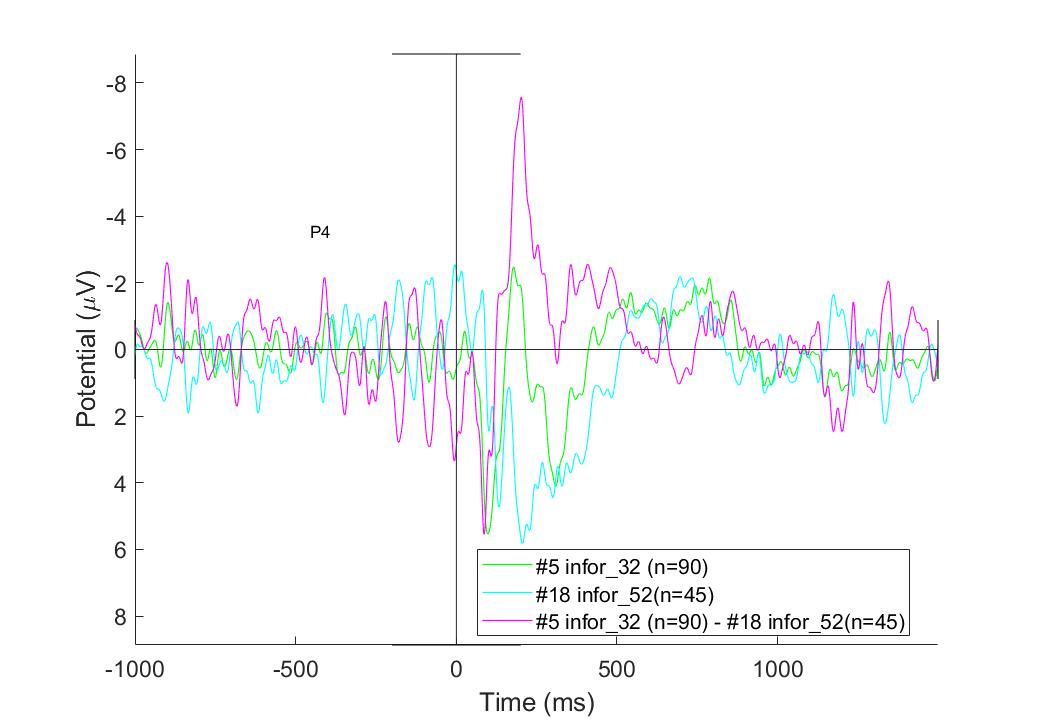
\includegraphics[width=.33\textwidth]{P43252.jpg}}
	\subfloat[PO3几何图形和花鸟图案ERP对比]{
		\label{fig:PO33252}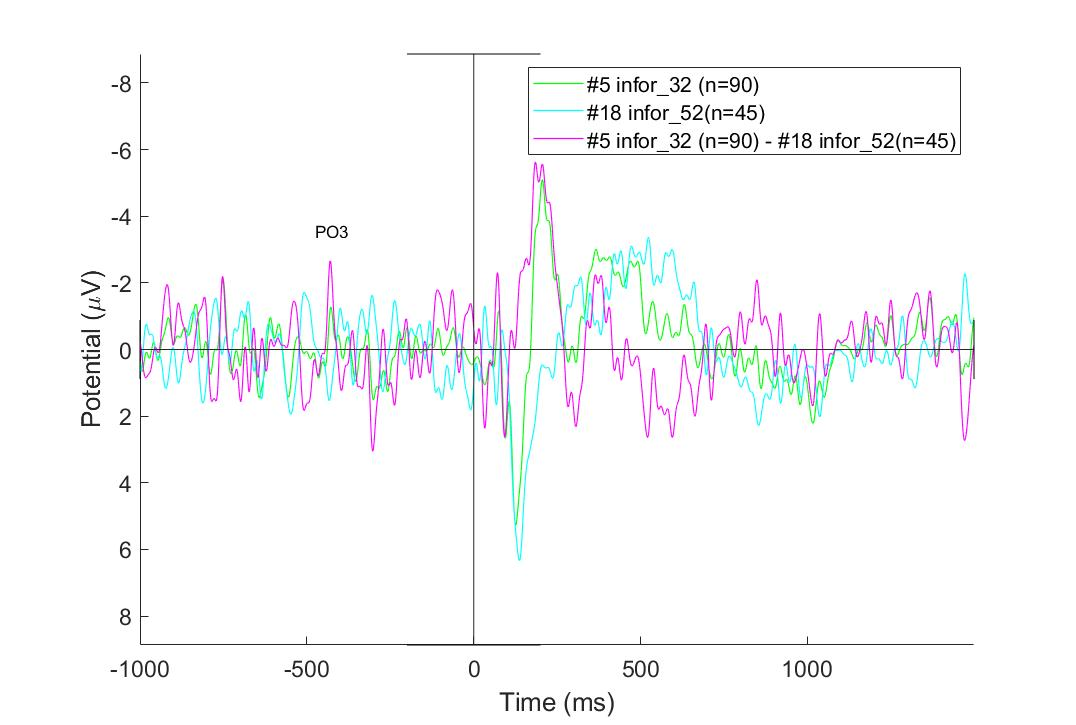
\includegraphics[width=.33\textwidth]{PO33252.jpg}}
	\\
	\subfloat[POZ几何图形和花鸟图案ERP对比]{
		\label{fig:POZ3252}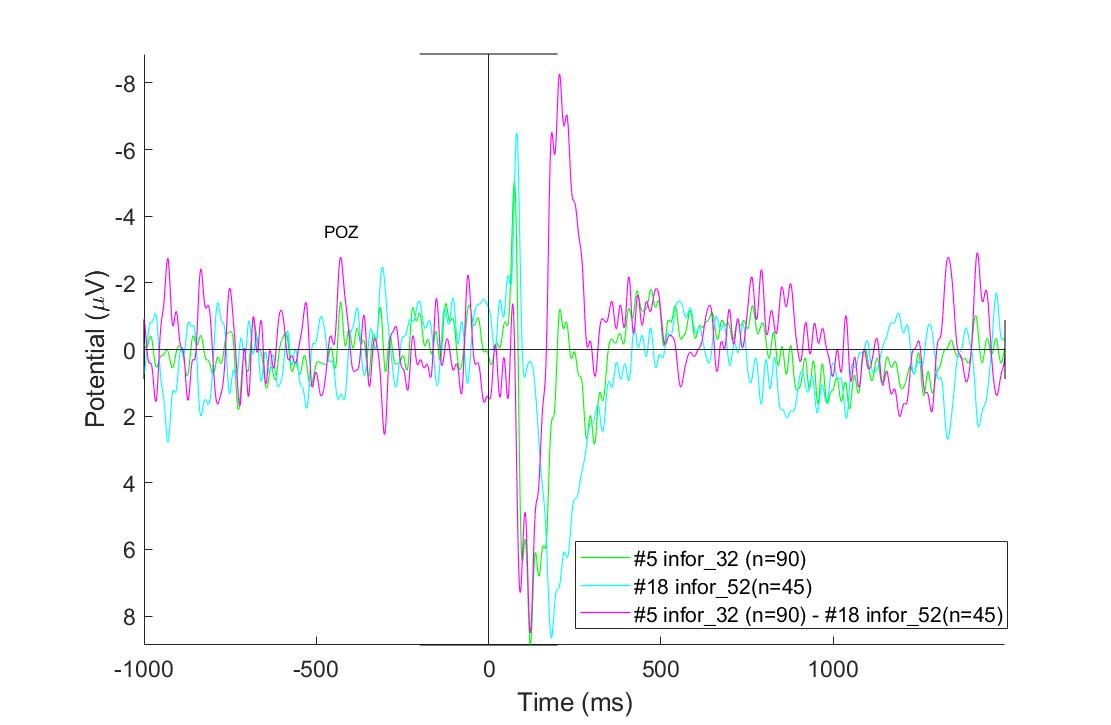
\includegraphics[width=.33\textwidth]{POZ3252.jpg}}
	\subfloat[PO4几何图形和花鸟图案ERP对比]{
		\label{fig:PO43252}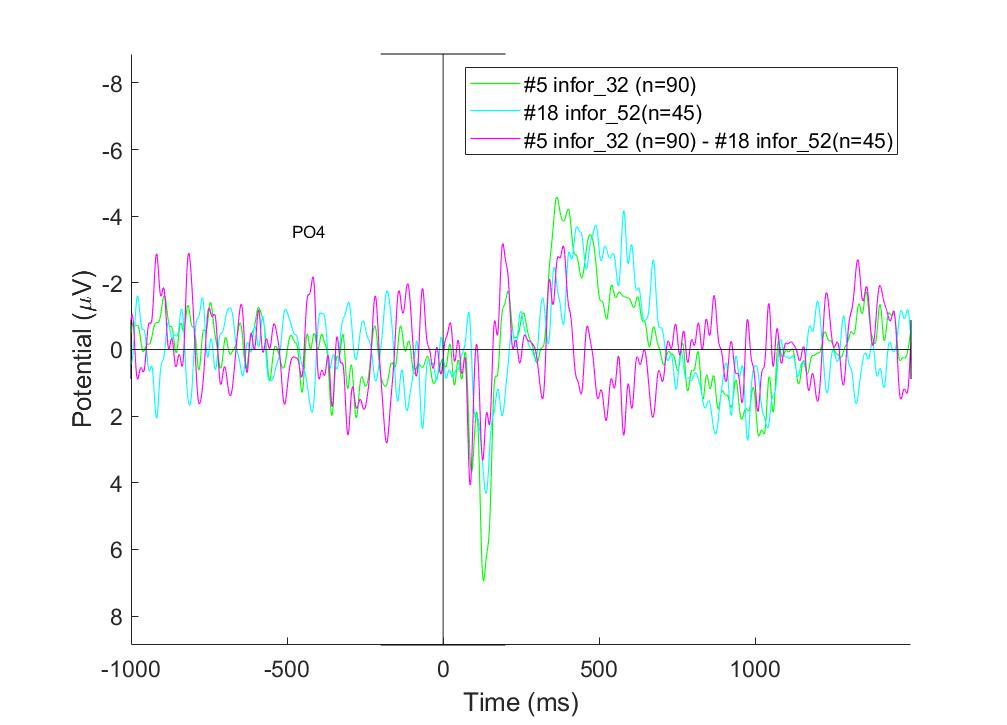
\includegraphics[width=.33\textwidth]{PO43252.jpg}}
	\subfloat[PO6几何图形和花鸟图案ERP对比]{
		\label{fig:PO63252}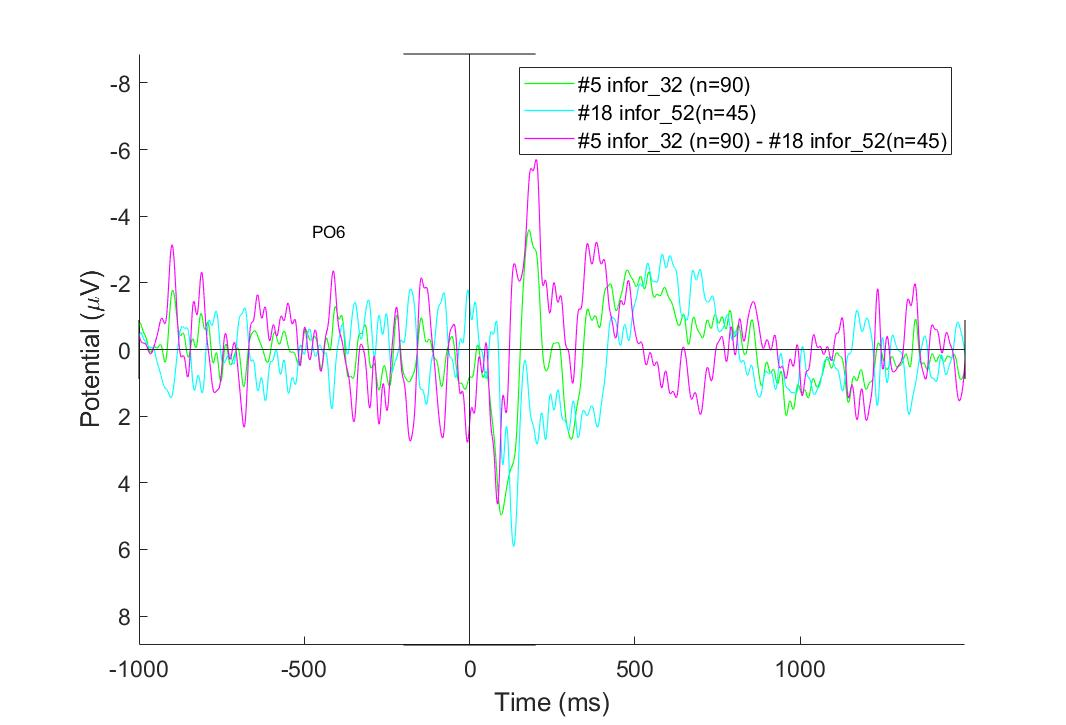
\includegraphics[width=.33\textwidth]{PO63252.jpg}}
\caption{有信息刺激时,右侧枕叶处相应电极的ERP对比结果}\label{fig:zhenye3252}
\end{figure}


此处几何图像的刺激以四个扇形的刺激为例。无信息刺激时,四个扇形图案完全随机分布引起的ERP结果如图(\ref{fig:infor41})所示,选择100、200、300、400、500、600、700、800、900ms时的ERP叠加图像,如图(\ref{fig:infor41detail})所示,可以看到在刺激发生后的100$\sim$300ms内,主要活跃的脑区为右侧枕叶,在400$\sim$800ms之间,主要活跃的脑区为左侧额叶和左侧顶叶;花鸟图案刺激引起的ERP结果如图(\ref{fig:infor53})所示,选择100、200、300、400、500、600、700、800、900ms时的ERP叠加图像,如图(\ref{fig:infor53detail})所示,可以看到在刺激发生后的100$\sim$500ms内,主要活跃的脑区为右侧枕叶和部分左侧枕叶,在700ms左右主要活跃的脑区为左侧额叶。二者对比是的ERP图像如图(\ref{fig:infor4153})所示,选择右侧枕叶和左侧顶叶附近的电极进行分析,右侧枕叶处相应电极的ERP叠加结果如图(\ref{fig:zhenye4153})所示,可以看到,在200ms左右,花鸟图案刺激下的右侧枕叶的ERP幅值要高于四个扇形图案引起的刺激,而且右侧枕叶ERP幅值较高持续时间较长,由此可以印证,右侧枕叶是对图像认知的能力较为活跃的区域;左侧额叶和左侧顶叶处相应电极的ERP叠加结果如图(\ref{fig:eye4153})所示,可以看到,在500ms左右,四个完全随机分布扇形图案刺激下的左侧顶叶和左侧额叶的ERP幅值要高于花鸟图案引起的刺激,由此可以印证,左侧顶叶和左侧额叶的部分区域是对操作理解的能力较为活跃的区域。

\begin{figure}[htb]
\centering
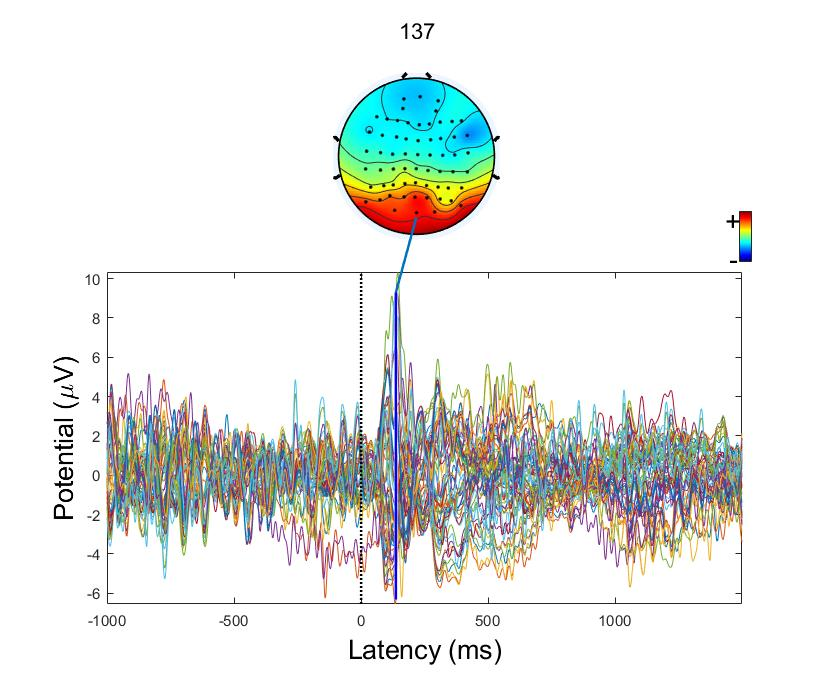
\includegraphics[scale=0.3]{infor41.jpg}
\caption{无信息刺激时,四个完全随机分布的扇形图案刺激的ERP结果}\label{fig:infor41}
\end{figure}

\begin{figure}[htb]
\centering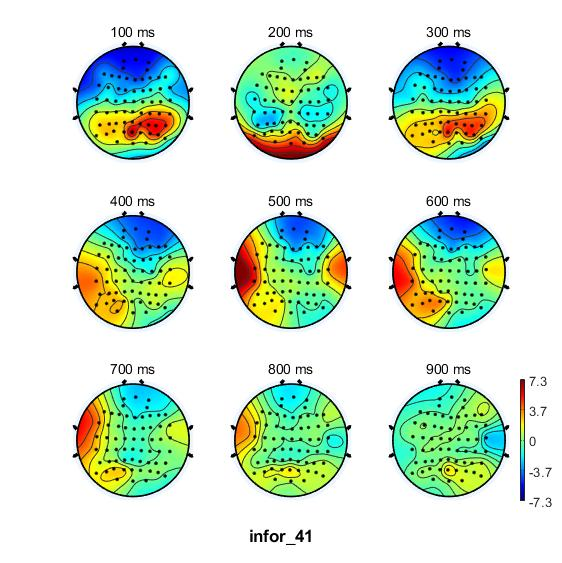
\includegraphics[scale=0.4]{infor41detail.jpg}
\caption{无信息刺激时,四个扇形完全随机分布的刺激的ERP分时结果}\label{fig:infor41detail}
\end{figure}

\begin{figure}[htb]
\centering
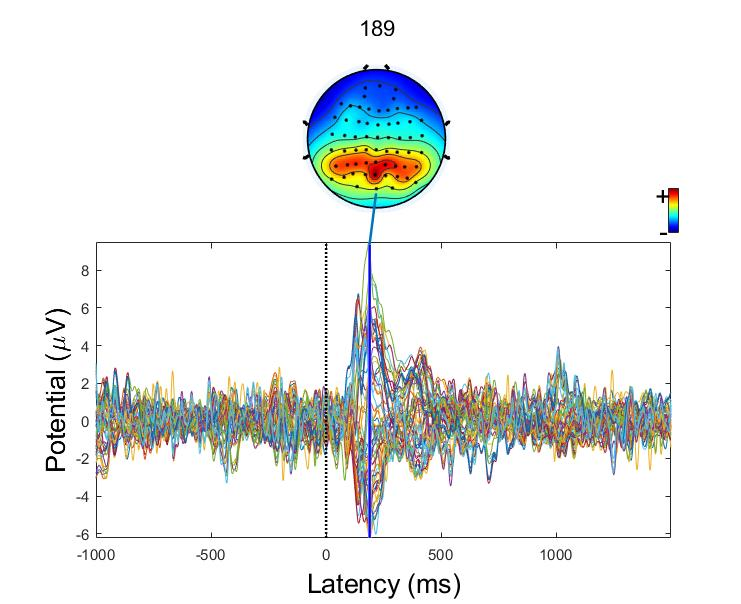
\includegraphics[scale=0.3]{infor53.jpg}
\caption{无信息刺激时,花鸟图案刺激的ERP结果}\label{fig:infor53}
\end{figure}

\begin{figure}[htb]
\centering
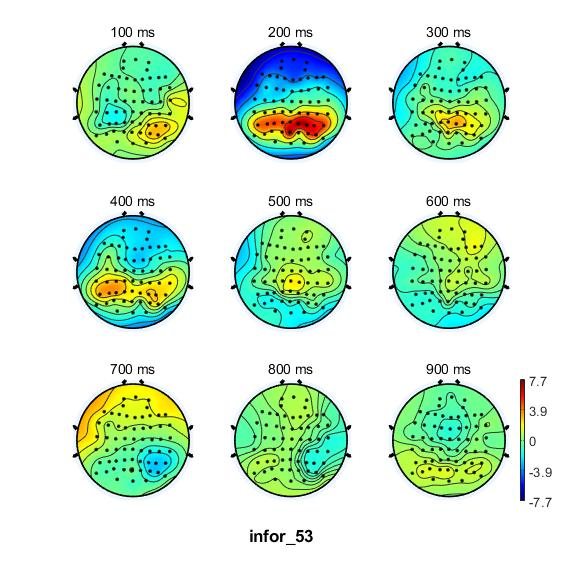
\includegraphics[scale=0.4]{infor53detail.jpg}
\caption{无信息刺激时,花鸟图案刺激的ERP分时结果}\label{fig:infor53detail}
\end{figure}

\begin{figure}[htb]
\centering
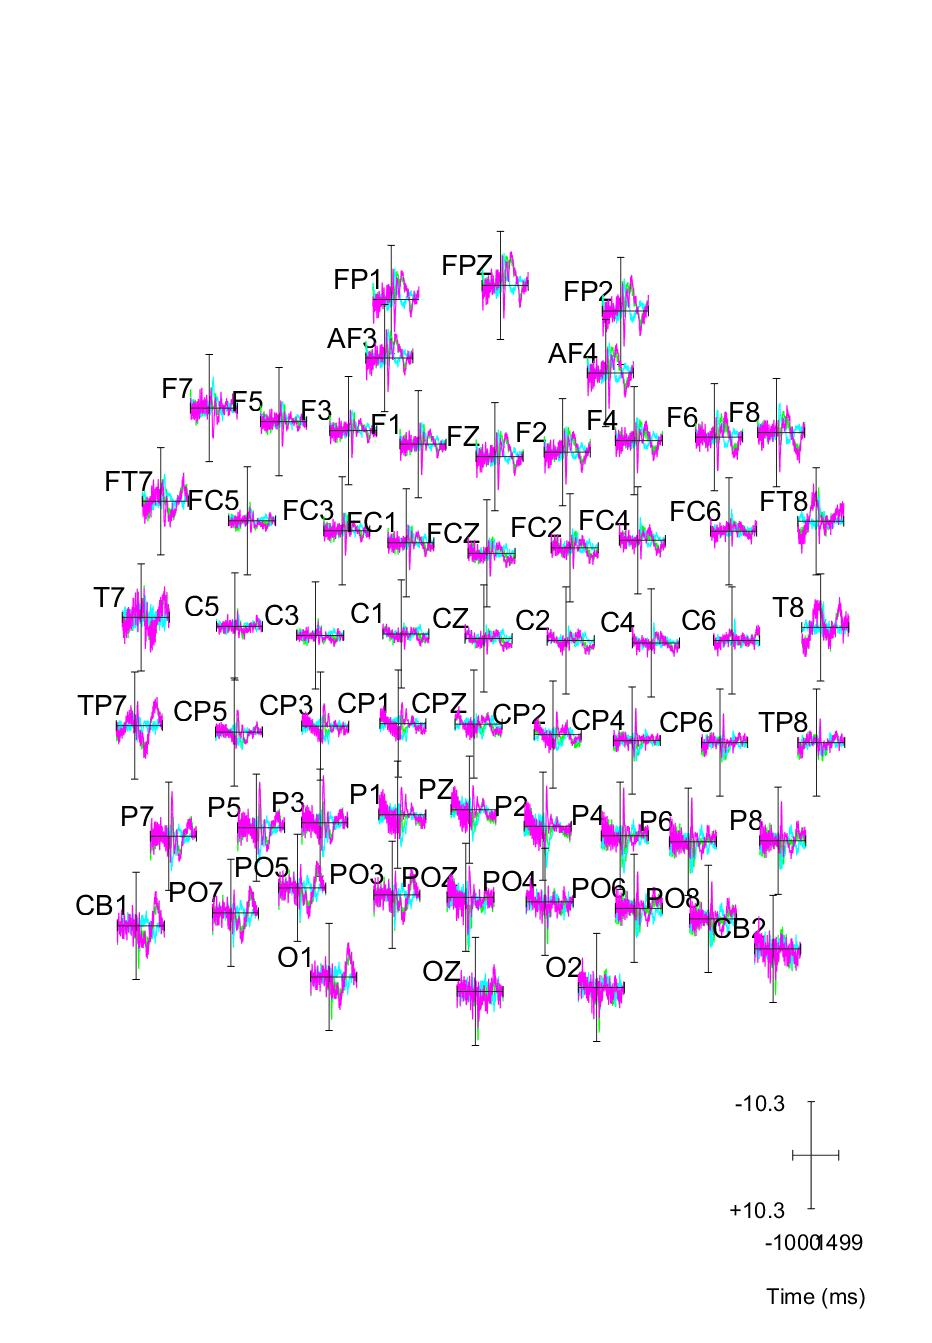
\includegraphics[height=0.4\textheight]{infor4153.jpg}
\caption{无信息刺激时,四个扇形图案完全随机分布的刺激与花鸟图案刺激的ERP比较}\label{fig:infor4153}
\end{figure}

\begin{figure}[htb]
\centering
	\subfloat[CP1电极几何图形和花鸟图案ERP对比]{
		\label{fig:CP14153}\includegraphics[width=.33\textwidth]{CP14153.jpg}}
	\subfloat[CPZ电极几何图形和花鸟图案ERP对比]{
		\label{fig:CPZ4153}\includegraphics[width=.33\textwidth]{CPZ4153.jpg}}
	\subfloat[CP2电极几何图形和花鸟图案ERP对比]{
		\label{fig:CP24153}\includegraphics[width=.33\textwidth]{CP24153.jpg}}
	\\
	\subfloat[CP4几何图形和花鸟图案ERP对比]{
		\label{fig:CP44153}\includegraphics[width=.33\textwidth]{CP44153.jpg}}
	\subfloat[P1几何图形和花鸟图案ERP对比]{
		\label{fig:P14153}\includegraphics[width=.33\textwidth]{P14153.jpg}}
	\subfloat[PZ几何图形和花鸟图案ERP对比]{
		\label{fig:PZ4153}\includegraphics[width=.33\textwidth]{PZ4153.jpg}}
	\\
	\subfloat[P2几何图形和花鸟图案ERP对比]{
		\label{fig:P24153}\includegraphics[width=.33\textwidth]{P24153.jpg}}
	\subfloat[P4几何图形和花鸟图案ERP对比]{
		\label{fig:P44153}\includegraphics[width=.33\textwidth]{P44153.jpg}}
	\subfloat[PO3几何图形和花鸟图案ERP对比]{
		\label{fig:PO34153}\includegraphics[width=.33\textwidth]{PO34153.jpg}}
	\\
	\subfloat[POZ几何图形和花鸟图案ERP对比]{
		\label{fig:POZ4153}\includegraphics[width=.33\textwidth]{POZ4153.jpg}}
	\subfloat[PO4几何图形和花鸟图案ERP对比]{
		\label{fig:PO44153}\includegraphics[width=.33\textwidth]{PO44153.jpg}}
	\subfloat[PO6几何图形和花鸟图案ERP对比]{
		\label{fig:PO64153}\includegraphics[width=.33\textwidth]{PO64153.jpg}}
\caption{无信息刺激时,右侧枕叶处相应电极的ERP对比结果}\label{fig:zhenye4153}
\end{figure}

\begin{figure}[htb]
\centering
	\subfloat[FT7电极几何图形和花鸟图案ERP对比]{
		\label{fig:FT74153}\includegraphics[width=.33\textwidth]{FT74153.jpg}}
	\subfloat[FC5电极几何图形和花鸟图案ERP对比]{
		\label{fig:FC54153}\includegraphics[width=.33\textwidth]{FC54153.jpg}}
	\subfloat[FC3电极几何图形和花鸟图案ERP对比]{
		\label{fig:FC34153}\includegraphics[width=.33\textwidth]{FC34153.jpg}}
	\\
	\subfloat[T7几何图形和花鸟图案ERP对比]{
		\label{fig:T74153}\includegraphics[width=.33\textwidth]{T74153.jpg}}
	\subfloat[C5几何图形和花鸟图案ERP对比]{
		\label{fig:C54153}\includegraphics[width=.33\textwidth]{C54153.jpg}}
	\subfloat[C3几何图形和花鸟图案ERP对比]{
		\label{fig:C34153}\includegraphics[width=.33\textwidth]{C34153.jpg}}
	\\
	\subfloat[TP7几何图形和花鸟图案ERP对比]{
		\label{fig:TP74153}\includegraphics[width=.33\textwidth]{TP74153.jpg}}
	\subfloat[CP5几何图形和花鸟图案ERP对比]{
		\label{fig:CP54153}\includegraphics[width=.33\textwidth]{CP54153.jpg}}
	\subfloat[CP3几何图形和花鸟图案ERP对比]{
		\label{fig:CP34153}\includegraphics[width=.33\textwidth]{CP34153.jpg}}
\caption{无信息刺激时,左侧额叶和左侧顶叶处相应电极的ERP对比结果}\label{fig:eye4153}
\end{figure}



\paragraph{问题三}~{}

根据问题二中得到的图(\ref{fig:infor32detail})和图(\ref{fig:infor52detail})与图(\ref{fig:infor41detail})和图(\ref{fig:infor53detail})的结果显示,在无信息刺激引起的ERP情况下,相应脑区的ERP幅值要较有信息刺激引起的ERP较高,可能是由于大脑需要对无信息作出更多的分析,导致了ERP信号幅值较高;此外,无信息刺激刺激会导致在500ms之后的信息确认阶段,相应脑区的ERP信号幅值较高,可能是大脑需要对无信息情况作出更肯定的确认,导致ERP信号幅值较高。

在判断是否有无信息时,根据实验结果的图(\ref{fig:infor52detail})和图(\ref{fig:infor41detail})显示,主要活跃的脑区为右侧枕叶,经查阅资料得知,此部分脑区与图像认知能力相关\cite{malenkachapter20151},实验得到的结果也可以佐证。在确认信息时,根据实验结果的图(\ref{fig:infor41detail})和图(\ref{fig:infor53detail})显示,主要活跃的脑区为左侧额叶的部分和左侧顶叶的部分,查阅资料得知,此部分脑区与操作理解能力相关\cite{malenkachapter20151},也可以通过实验证实。


\paragraph{问题四}~{}

\begin{enumerate}
\item ERP signs of categorical and supra-categorical processing of visual information\cite{Zani2015}

\hspace{2em}本文研究的目的是调查在多大程度上共享和不同的大脑机制可能有助于视觉超分类和分类知识观察与处理而产生的ERPs。并且对这些知识类型的获取时间也进行了调查。实验展示了动物、物体和混合类型的图片对。受试者被要求通过按下两个按钮中的一个来决定每对图片是属于同一类别(动物还是人造物体)还是属于不同类别。同时记录反应准确度和反应时间(RTs)。

\hspace{2em}对于相同、不同的超类别和动物-物体类别,分别对受试者的ERP和RTs进行了总平均。对于ERPs,发现了对相同和不同的超分类对的最早C1和随后的P1反应的调节,但对动物和物体两种类别对的调节不明显。这一发现支持这样一种观点,即纹状体皮层的早期传入加工可以作为注意力分配到形状和基本特征加工的副产品而得到促进,这些形状和基本特征在相同-不同的超分类判断过程中不匹配,但不匹配它们的语义精髓。最重要的是,这种加工累积的发生独立于传统的实验条件,这种实验条件要求从所述的各种刺激源中选择性地注意刺激源,这种加工累积可能产生于视觉注意交替聚焦所产生的注意需求刺激范畴对的基本结构特征。

\hspace{2em}实验结果表明,当前的ERP结果揭示了共享的和不同的机制来访问超分类知识和分类知识,而共享和独特的神经表示是处理各种语义类别的基础。此外,本文还简述了分类和超分类表示的序列性质,指示了访问这些单独的知识类型的顺序步骤。

\item Semantic integration of differently asynchronous audio–visual information in videos of real-world events in cognitive processing: An ERP study\cite{Liu2011}

\hspace{2em}本文采用ERPs分析方法研究认知加工中不同异步视听信息的语义整合。受试者被呈现真实世界事件的视频,其中听觉和视觉信息是暂时不同步的。当关键动作在声音之前时,与前面的关键动作不一致的声音与一致的条件相比会产生N400效应。实验结果表明,N400索引的语义-语境整合同样适用于多感官信息的认知加工。此外,与其他视觉诱发的N400研究相比,N400效应在潜伏期早期。结果表明,与孤立的视觉信息相比,跨模式信息在时间上得到了促进。当声音先于关键动作时,与不协调状态相比,在不协调状态下观察到较大的后期正波。 P600可能代表重新分析过程,其中评估了关键动作和先前声音之间的不匹配。实验得到结论,环境声音可能会影响视觉事件的认知过程。

\item Integration of sensory information precedes the sensation of vection: A combined behavioral and event-related brain potential (ERP) study\cite{Keshavarz2014}

\hspace{2em}Illusory self-motion描述了缺乏身体运动时自我运动的感觉。无意识的运动行为通常发生在暴露于暗示自我运动的视觉信息(例如模拟器,虚拟现实)中静止的观察者身上。在本研究中测试了视觉信息的感官整合是否会触发运动,13位受试者在屏幕上被分为中心视野和周围视野中移动的黑白垂直条纹感知移动。当条纹的固定中心被移动的外围包围时,受试者显示出明显更可能的运动倾向。根据实验数据,周围和中央视觉信息的感觉整合触发了对运动的感知。

\hspace{2em}实验结果表明,运动处理的反馈是非常快的,在视觉处理开始约150毫秒后就会进行运动信息的处理。其次,实验发现,刺激类型影响P1和N2在不同的方式表现不同。这表明,多个神经循环网络并行处理,并影响视觉信息处理的不同步骤。最后,实验将重点放在水平方向上的平移运动上,因为这种情况特别能够引发较为明显的运动倾向。在扩展研究评估这种刺激的矢量,我们应用了一个评分量表,不仅评估运动行为发生,而且还评估了运动的强度。有趣的是,N2分量的振幅随矢量强度的变化而变化,也就是说,我们发现运动趋势最强时N230最明显,运动趋势最弱时N230最小。此外,还发现有证据表明,在实际发生运动之前,神经过程先于对运动强度的主观感知。

\item The automatic processing of visual information at different visual acuity levels: An ERP study\cite{Meng2015}

\hspace{2em}本研究通过记录与任务无关的视觉变化诱发的事件相关电位ERPs来研究主观视力。视阈刺激呈现在三个阈值水平(超阈值、阈值附近和亚阈值)的视野中心,同时参与者需要听一些相关信息。结果表明,视型刺激在亚阈值条件下不诱发vmmn和P3a成分,而在超阈值和阈值附近条件下均不诱发vmmn,两种条件下的vmmn振幅无显著差异。超阈值条件下的P3a幅度大于阈值条件下的。 这些数据表明,vMMN的出现仅反映了与低于阈值条件相比超阈值和阈值条件中方向变化的自动检测,而P3a振幅可能反映了高于阈值和阈值的处理差异 刺激。

\hspace{2em}本文的研究证明了关于视敏度与ERP组件之间相关性的初步想法。实验发现,vMMN只能反映自动检测超阈值和阈值附近的变化,而不能反映ERP的更高或更好的处理成分;相反,P3a可以反映更高的处理水平,这与每个视敏度级别的信息容量有关。通过分析在三种视敏度条件下引起的vMMN和P3a成分的不同特征,合理地提出人脑能够在相对非注意条件下检测可见视标的观点。

\item RP and N400 ERP components reflect semantic violations in visual processing of human actions\cite{Proverbio2009}

\hspace{2em}本文基于ERPs研究人类典型动作的视觉加工。研究人员向23名右利手学生展示了260幅彩色图片,这些图片代表了不同人数、年龄和性别的人,图片中的人物在做一些简单的活动。对有意义行为的认知(例如,年轻女子在商店试鞋)与对缺乏可理解目标的行为的认知(例如,女商人在沙漠中单脚平衡)形成对比。结果表明,早期识别的可理解行为的形式增强后“识别潜力”(RP)(N250),其次是更大的消极(N400)的反应不一致的行动。结果表明,从概念的角度来看,与人的手势有关的传入视觉信息的处理方式与语言输入类似。因此,当动作代码被视觉识别和理解时,会产生一个后验RP,而在未识别到或未识别到动作时引发了N400,难以与先验知识相结合。



\end{enumerate}


\newpage

\renewcommand\refname{参考文献}
 
\bibliographystyle{unsrt} %%参考文献的格式(可选的格式还有:plain)
 
\bibliography{Reference.bib}    %%参考文件存储位置

\newpage
\begin{appendices}

\section{处理oddball听觉实验数据——oddball.py}\label{app:oddball}

\lstinputlisting[language=python]{../src/oddball.py}

\section{处理信息处理实验数据——information\_cognition.py}\label{app:information}

\lstinputlisting[language=python]{../src/information_cognition.py}
%
%\section{对语料端点检测——voice\_endpoint\_detection.py}
%
%\lstinputlisting[language=python]{code/voice_endpoint_detection.py}
%
%\section{将语音短时能量、过零率、端点检测结果写入文件——write\_to\_file.py}
%
%\lstinputlisting[language=python]{code/write_to_file.py}

\end{appendices}

\end{document}
